\documentclass[aspectratio=169]{beamer} 

\usepackage{hayesmacros}
\usepackage{appendixnumberbeamer}
\usepackage{subcaption}
\usepackage{caption}

\usetheme[numbering=none, block=fill]{metropolis}
\setsansfont{Fira Sans}  % be sure to compile with XeLaTeX

\usepackage{natbib}
\usepackage{ulem}
\usepackage{fontawesome5}

\newtheorem{proposition}{Proposition}
\newtheorem{assumption}{Assumption}

\theoremstyle{remark}
\newtheorem*{remark}{Remark}

\setbeamercolor{background canvas}{bg=white}
\setbeamercolor{normal text}{fg=black}
\setbeamercolor{frametitle}{bg=black, fg=white}

\hypersetup{colorlinks,citecolor=cyan, urlcolor=cyan, linkcolor=black}

\title{Estimating network-mediated causal effects via
spectral embeddings}

% Principle components network regression for causal inference with network embeddings
% Causal Network Influence with Latent Homophily and Measurement Error: An Application to Therapeutic Community
% Linear regression and its inference on noisy network-linked data
% Linear regression for causal inference on social networks via network embeddings

\date{NetSci 2024}
\author{Alex Hayes}
\institute{Department of Statistics \\ University of Wisconsin-Madison}

\begin{document}

\maketitle

\begin{frame}{This is joint work}
    \begin{columns}
        \centering
        \begin{column}{0.5\textwidth}
            \begin{figure}
                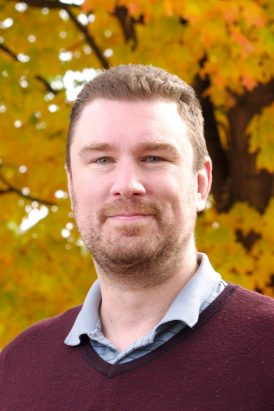
\includegraphics[width=4cm, height=5.75cm]{./figures/mark.jpg}
            \end{figure}
            \centering
            Mark Fredrickson \\
            University of Michigan
        \end{column}
        \begin{column}{0.5\textwidth}
            \centering
            \begin{figure}
                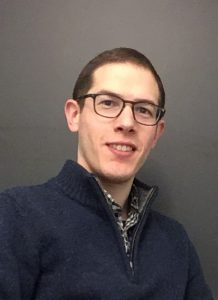
\includegraphics[width=4cm, height=5.75cm]{./figures/keith.jpg}
            \end{figure}
            Keith Levin \\
            UW-Madison
        \end{column}
    \end{columns}
\end{frame}

\begin{frame}{Motivation: understand causes of teenage smoking \citep{michell1996}}
    \begin{columns}
        \centering
        \begin{column}{0.55\textwidth}
            \begin{figure}
                \centering
                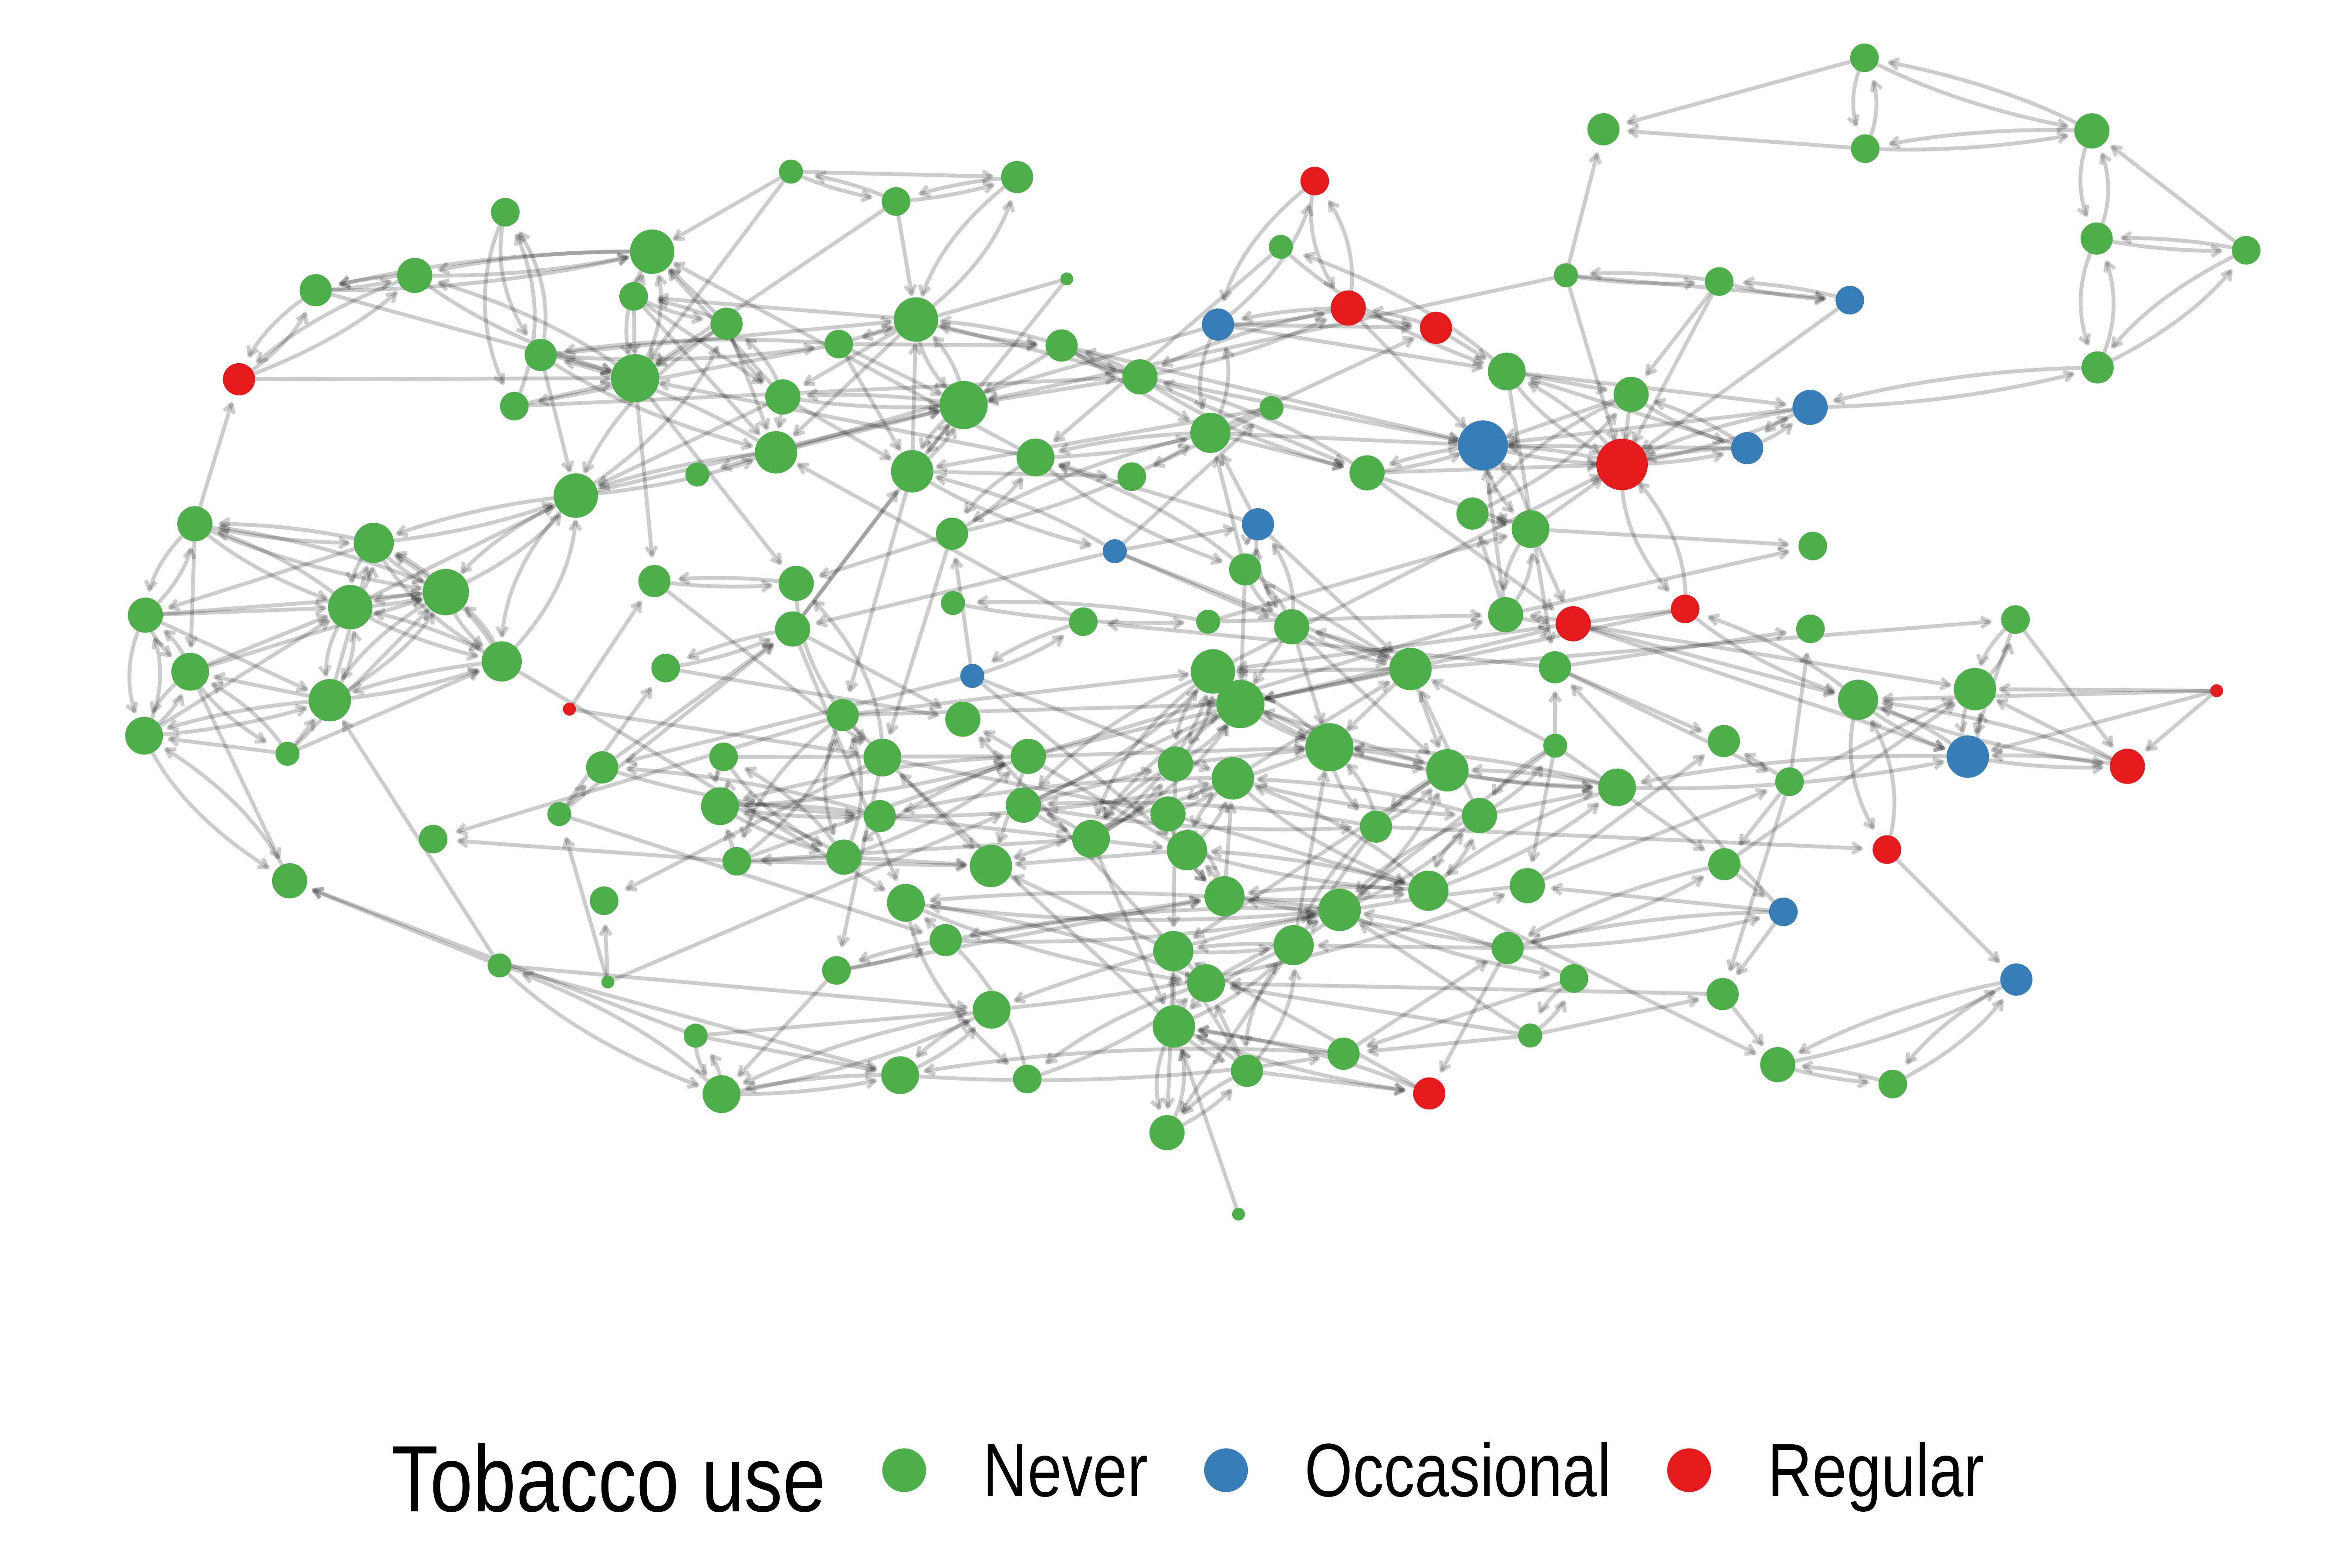
\includegraphics[width=1.05\textwidth]{figures/glasgow/tobacco.png}
            \end{figure}
        \end{column}
        \begin{column}{0.5\textwidth}
            \begin{itemize}
                \item 129 middle-schoolers in Glasgow
                \item {\bf Social network} based on self-reported friendships
                \item {\bf Auxiliary data:} spending money, leisure activities
                \item {\bf Demographics:} sex, age
                \item {\bf Behavior:} alcohol, cannabis and tobacco use
            \end{itemize}
        \end{column}
    \end{columns}
    \vspace{2mm}
    \pause
    \centering
    \textbf{Question:} how does sex influence tobacco use?
\end{frame}

\begin{frame}{Smoking is a sexually differentiated behavior and also a social behavior}
    \begin{columns}
        \centering
        \begin{column}{0.55\textwidth}
            \begin{figure}
                \centering
                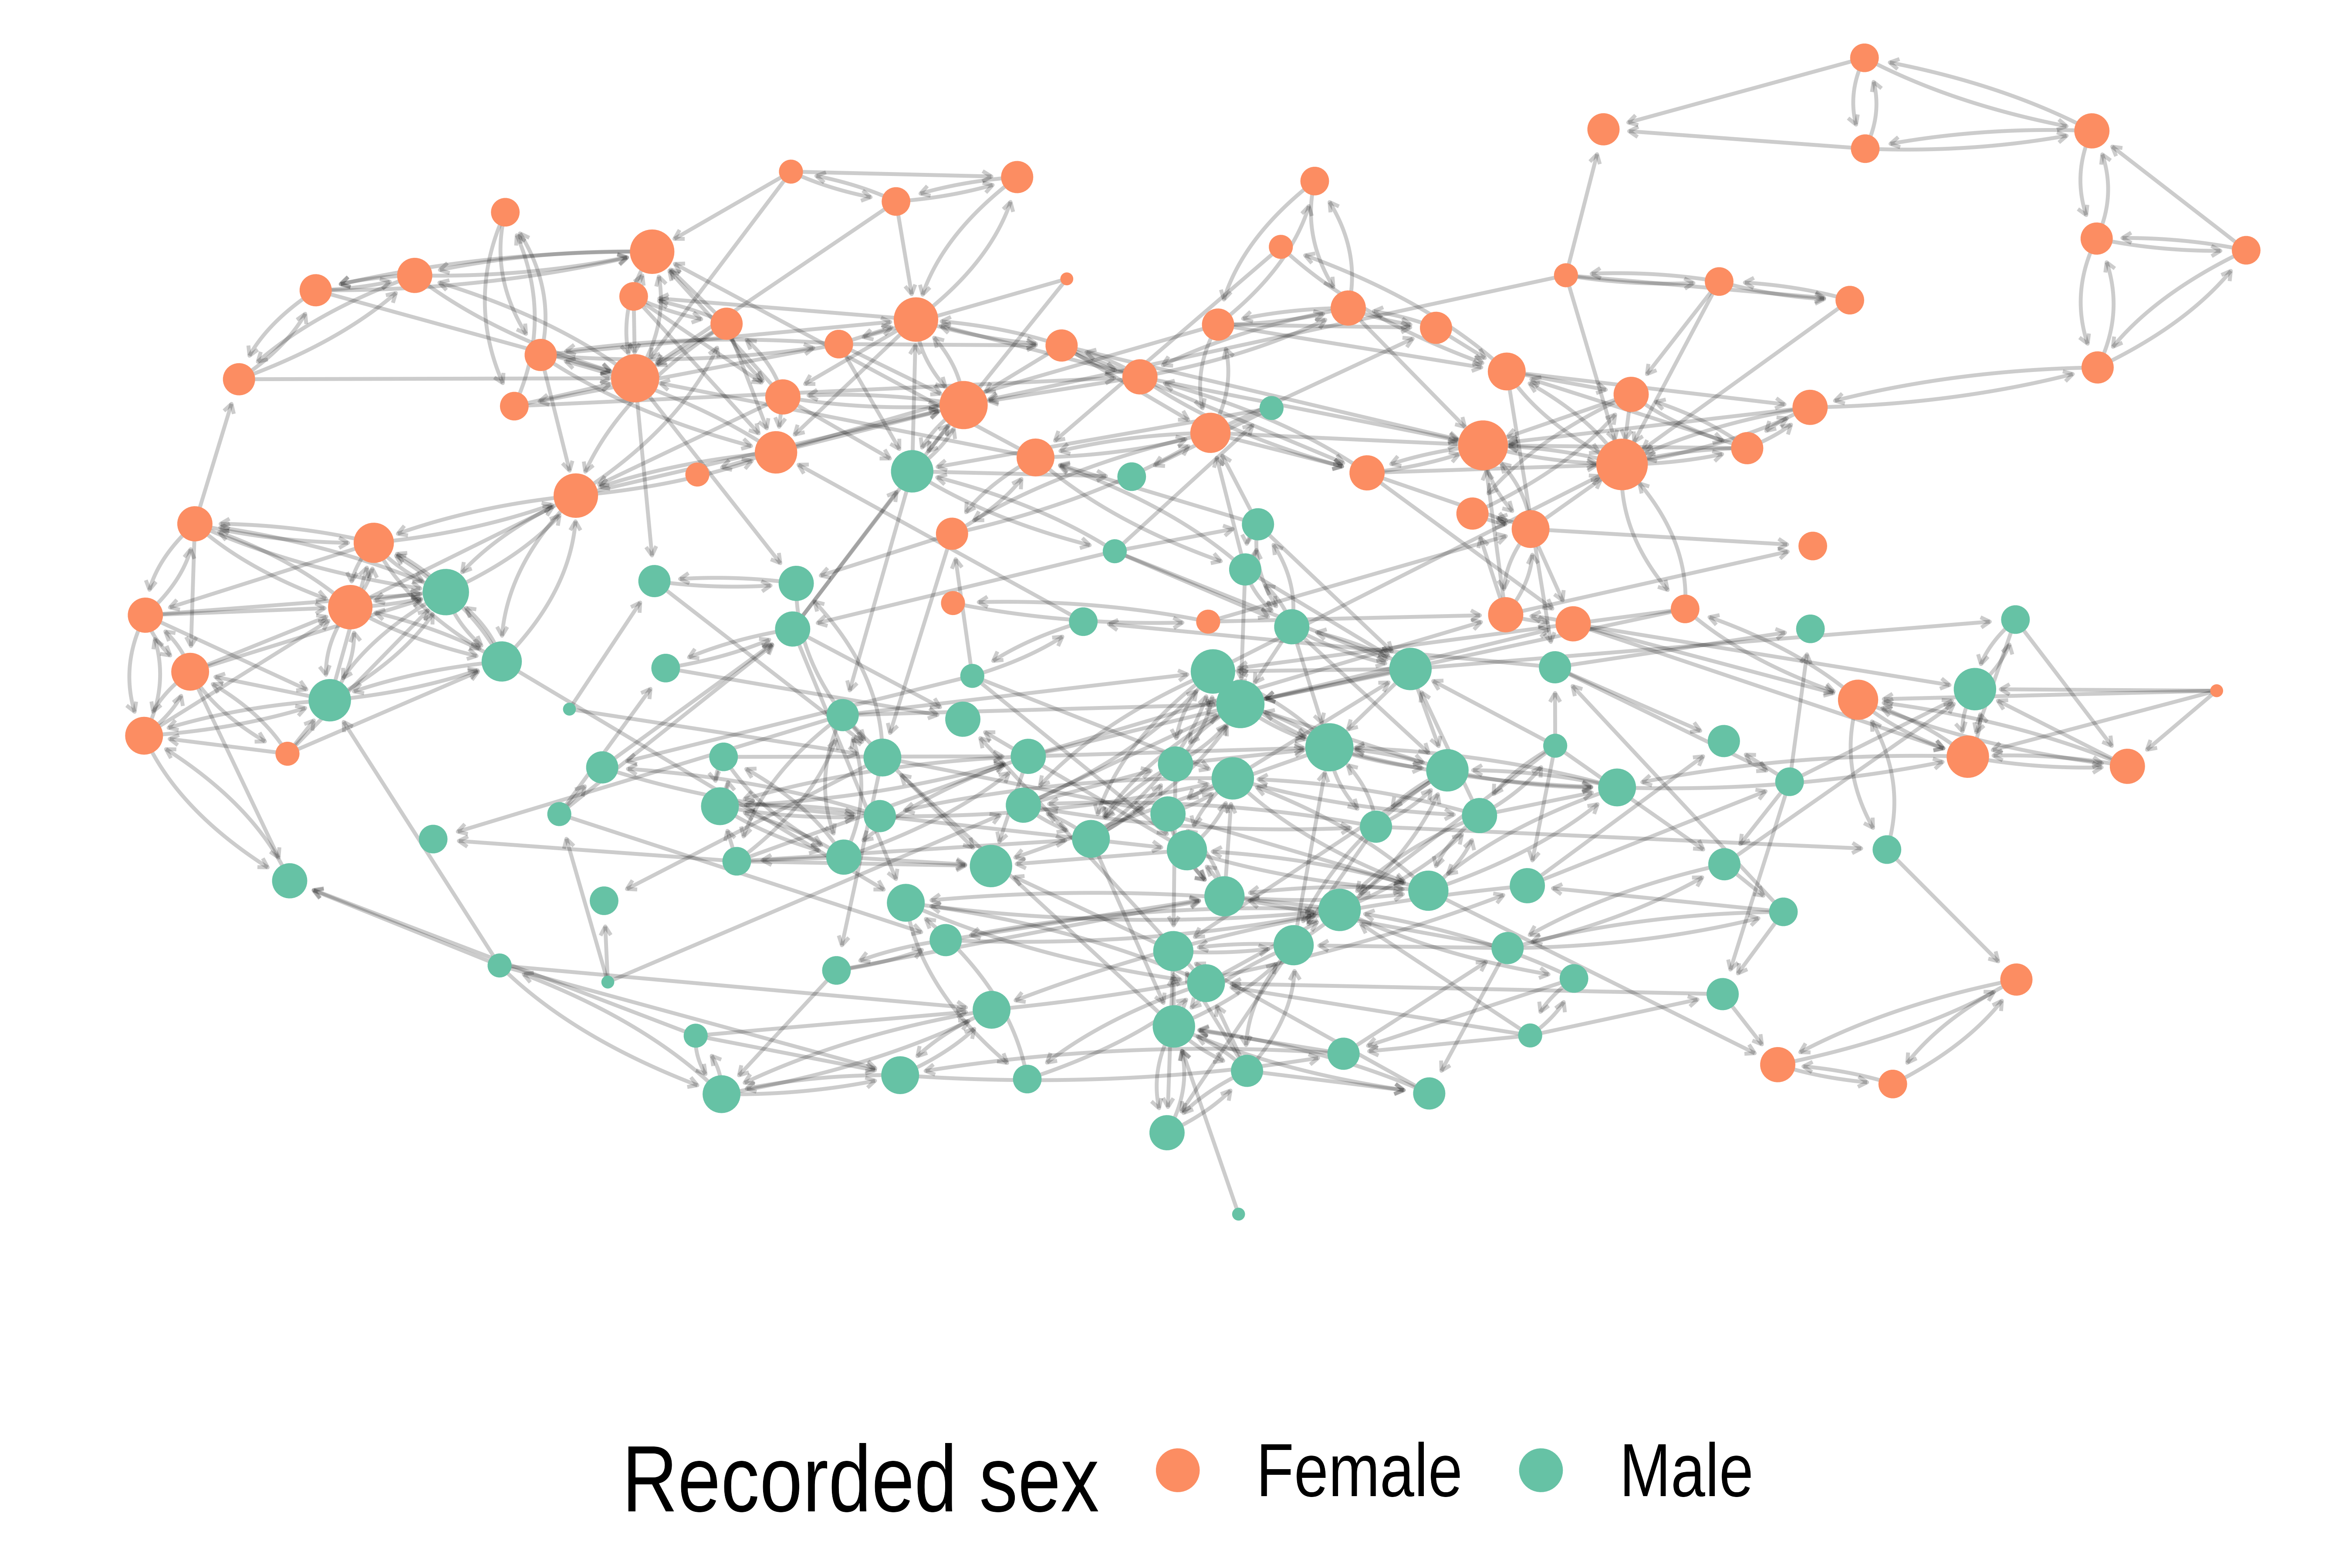
\includegraphics[width=1.05\textwidth]{figures/glasgow/sex.png}
            \end{figure}
        \end{column}
        \begin{column}{0.5\textwidth}
            \textbf{Direct effect} of sex on smoking
            \begin{itemize}
                \item Social and cultural expectations could lead to more or less smoking
            \end{itemize}
            \vspace{2mm}
            \textbf{Indirect effect} of sex on smoking
            \begin{itemize}
                \item Students tend to be friends with other students of same sex...
                \item ...friends induce one another to smoke
            \end{itemize}
        \end{column}
    \end{columns}
    \vspace{2mm}
    \pause
    \centering
    Should anti-smoking interventions target the direct or the social mechanism?
\end{frame}

\begin{frame}{Defining causal effects is straightforward when there is no social network}
    \begin{columns}
        \begin{column}{0.65\textwidth}
            \begin{table}[]
                \begin{tabular}{lrl}
                    Treatment   & $T_i$          & $\in \set{0, 1} $     \\
                    Outcome     & $Y_i$          & $\in \R$              \\
                    Mediators   & $\X_{i \cdot}$ & $\in \R^{1 \times d}$ \\
                    Confounders & $C_{i \cdot}$  & $\in \R^{1 \times p}$
                \end{tabular}
            \end{table}
        \end{column}
        \begin{column}{0.35\textwidth}
            \centering
            \begin{figure}[ht]
                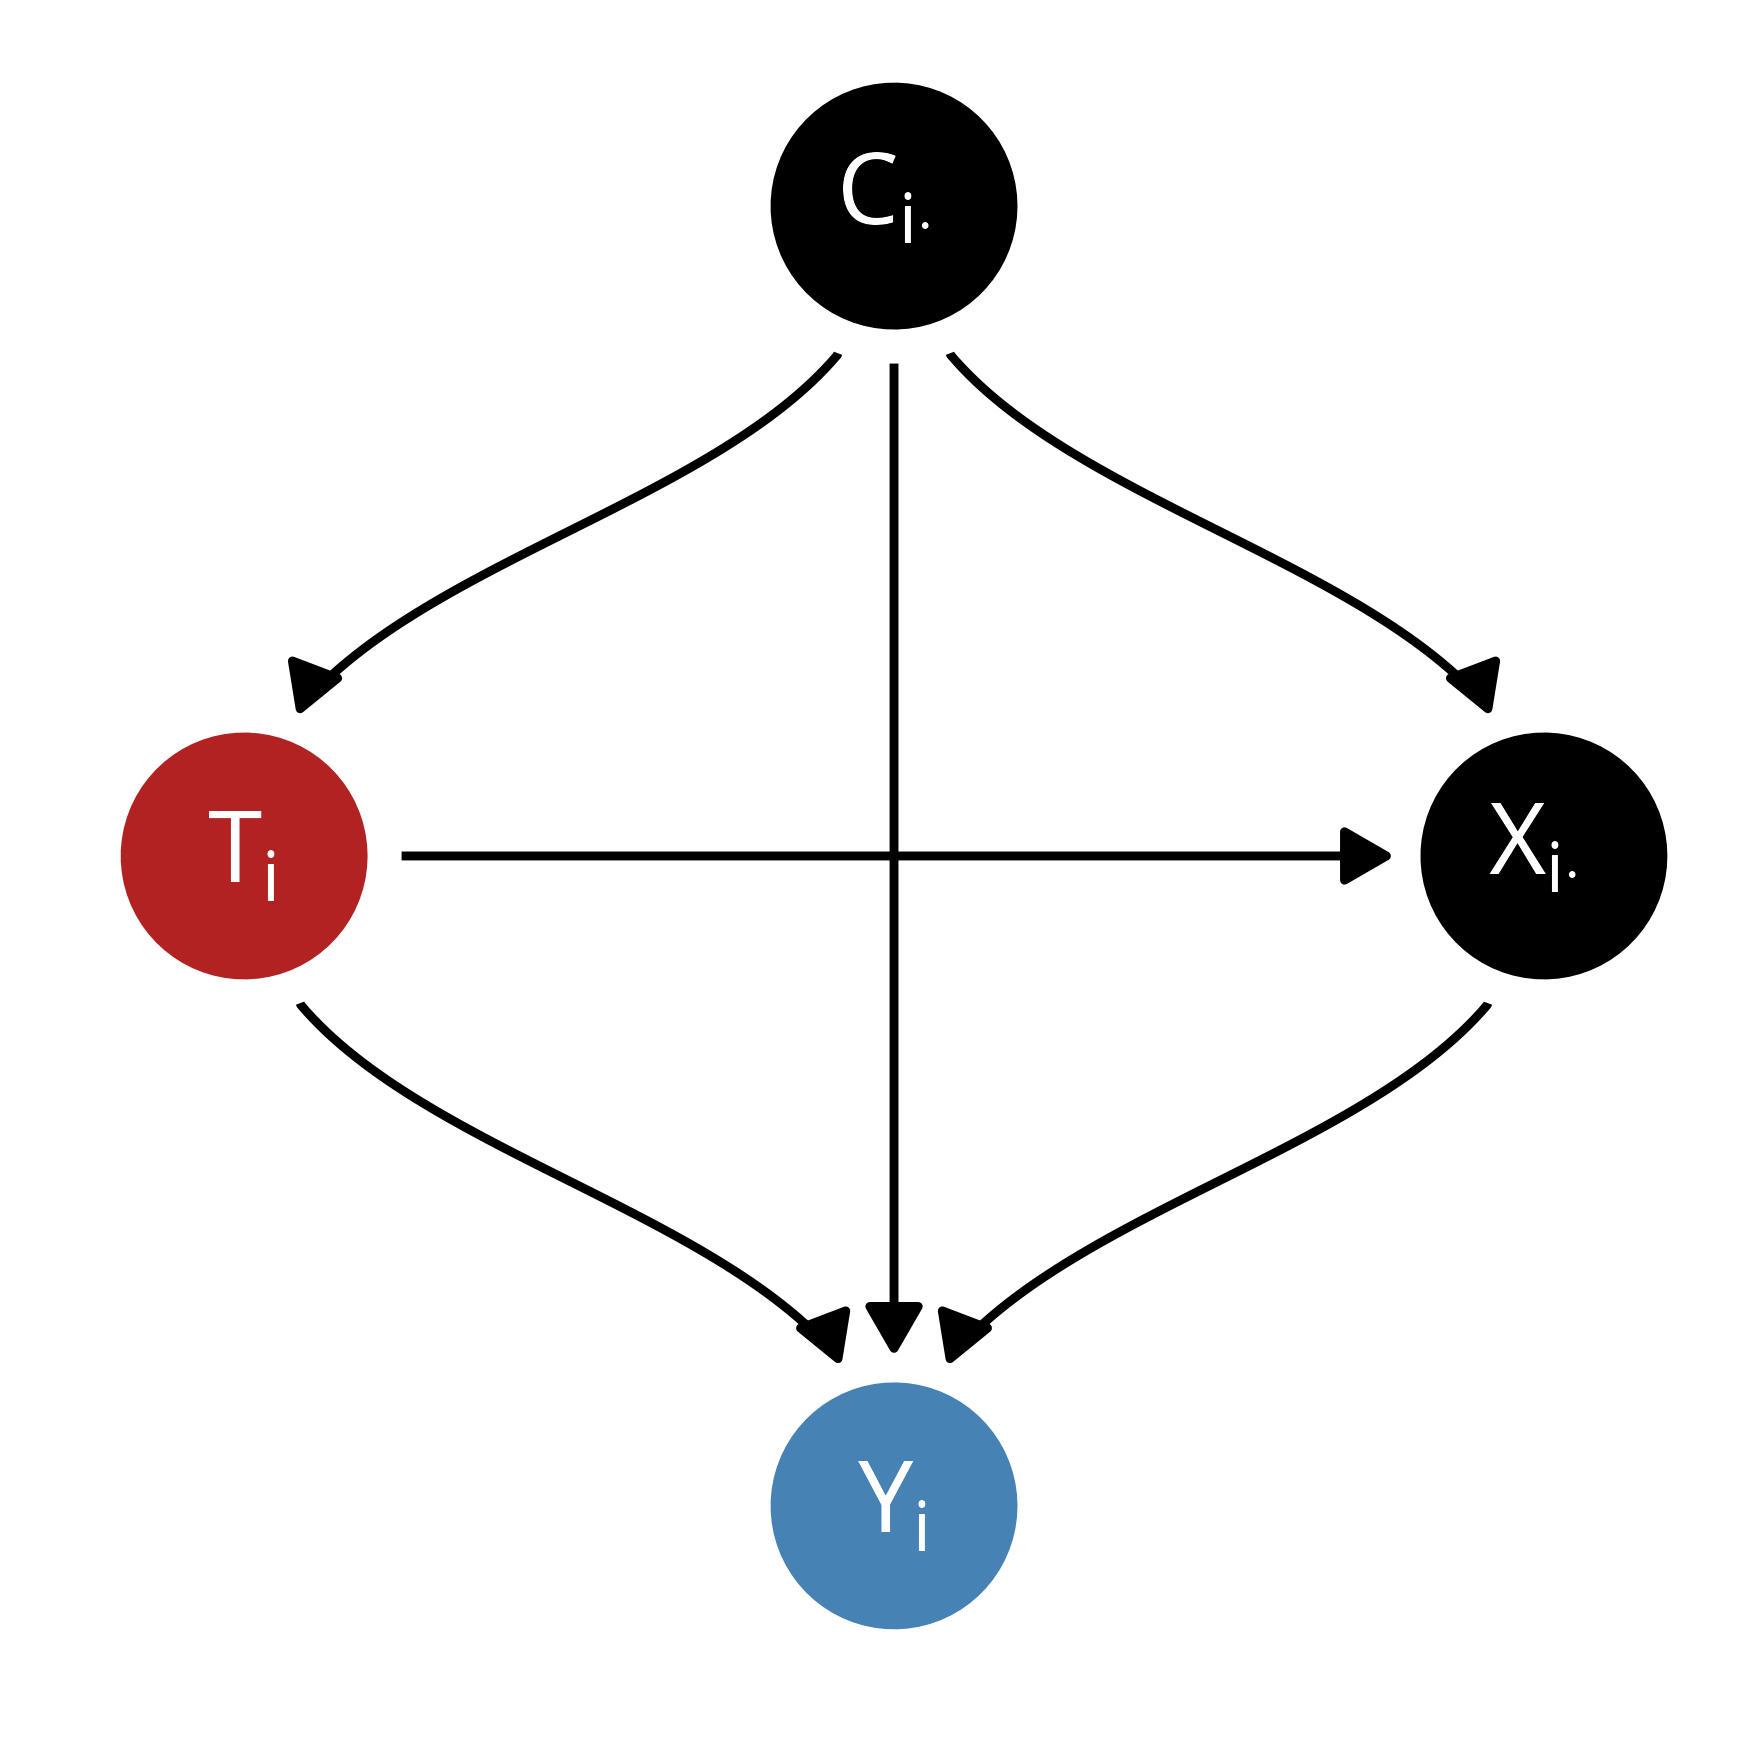
\includegraphics[height=0.5\textheight]{figures/dags/mediating.png}
            \end{figure}
        \end{column}
    \end{columns}
    \begin{definition}[Average treatment effect]
        \begin{equation*}
            \ate = \E{Y(1) - Y(0)}
        \end{equation*}
        \centering
        $Y(t)$ is the \underline{counterfactual outcome} under treatment value $t \in \{0, 1\}$.
    \end{definition}
\end{frame}

\begin{frame}{Decomposing causal effects is straightforward when there is no social network}
    \begin{columns}
        \begin{column}{0.65\textwidth}
            Two distinct mechanisms:
            \begin{enumerate}
                \item Direct effect along $T_i \to Y_i$ path
                \item Indirect effect along $T_i \to \X_{i \cdot} \to Y_i$ path
            \end{enumerate}
        \end{column}
        \begin{column}{0.35\textwidth}
            \centering
            \begin{figure}[ht]
                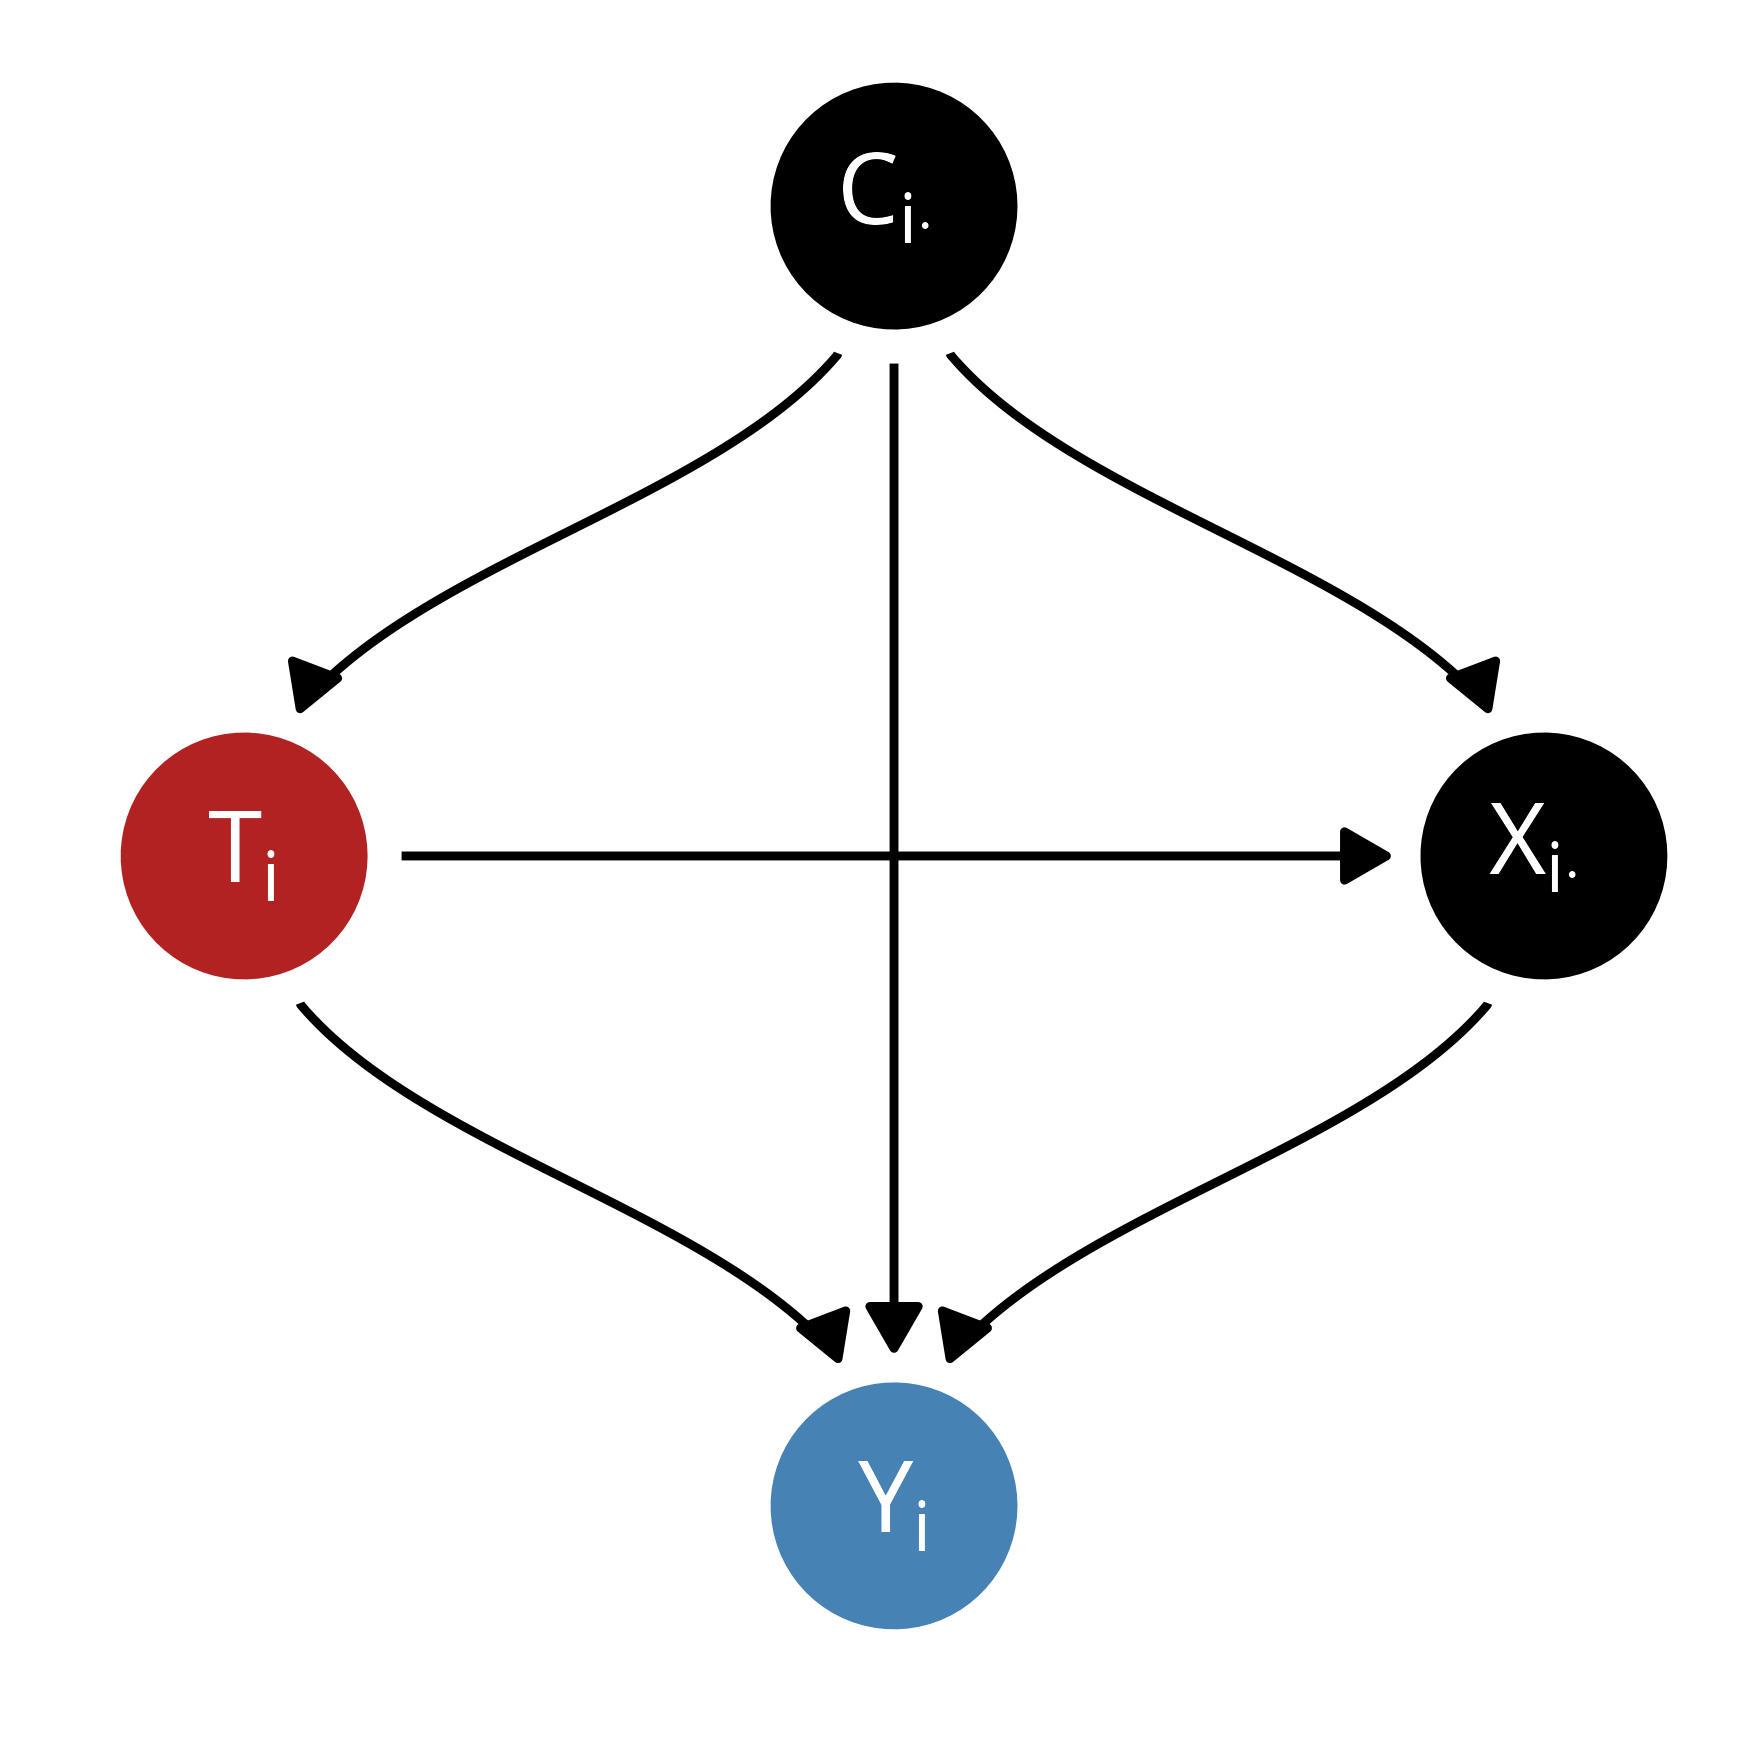
\includegraphics[height=0.5\textheight]{figures/dags/mediating.png}
            \end{figure}
        \end{column}
    \end{columns}
    \begin{definition}[Natural direct and indirect effects]
        \begin{equation*}
            \begin{aligned}
                \ate & = \nde + \nie                                               \\
                     & = \E{Y(1, X(0)) - Y(0, X(0))} + \E{Y(1, X(1)) - Y(1, X(0))}
            \end{aligned}
        \end{equation*}
        \centering
        $Y(t, m)$ is the \underline{counterfactual outcome} under treatment $t$ and mediator $m$
    \end{definition}
\end{frame}

\begin{frame}{We want to decompose node-level effects into direct and social components}
    \begin{columns}
        \begin{column}{0.4\textwidth}
            \begin{figure}
                \centering
                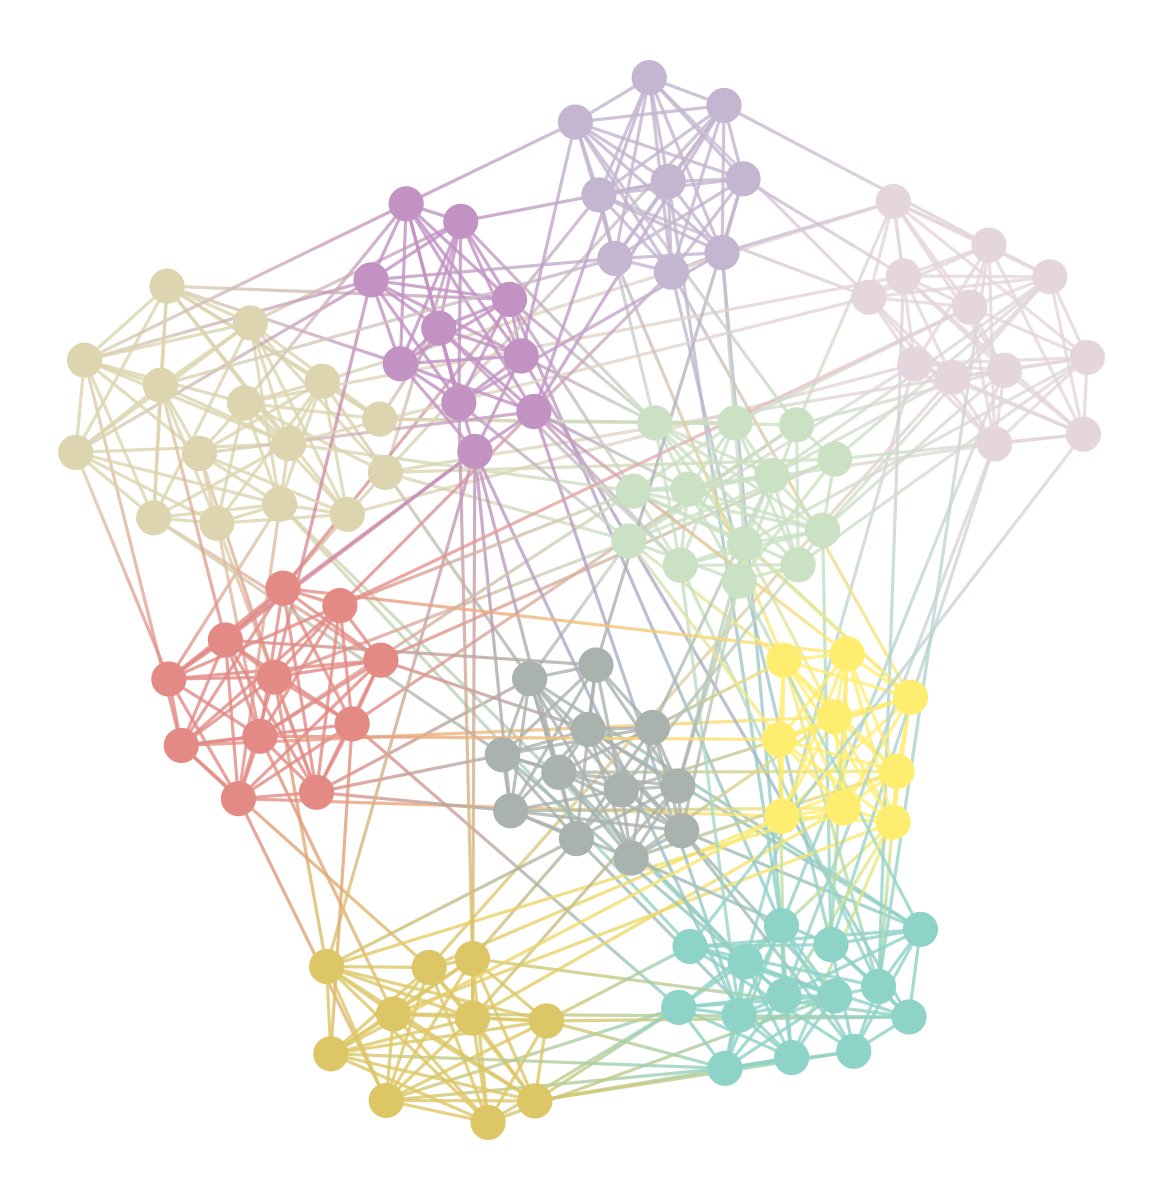
\includegraphics[width=\textwidth]{./figures/assortative.png}
            \end{figure}
        \end{column}
        \begin{column}{0.6\textwidth}
            Network $A \in \R^{n \times n}$ \\
            \vspace{2mm}
            For each node $i$:
            \begin{itemize}
                \item Treatment $T_i \in \{0, 1\}$
                \item Outcome $Y_i \in \R$
                \item Confounders $C_{i \cdot} \in \R^p$
            \end{itemize}
            \vspace{2mm}
            The network $A$ is noisy and complex but often exhibits high levels of homophily \\
            \vspace{2mm}
            \pause
            Assume each node belongs to a social group $\X_{i \cdot}$ and behaviors vary with social group
        \end{column}
    \end{columns}
\end{frame}


\begin{frame}{Stochastic blockmodels are the canonical model for social groups}
    \begin{columns}
        \begin{column}{0.4\textwidth}
            \begin{figure}
                \centering
                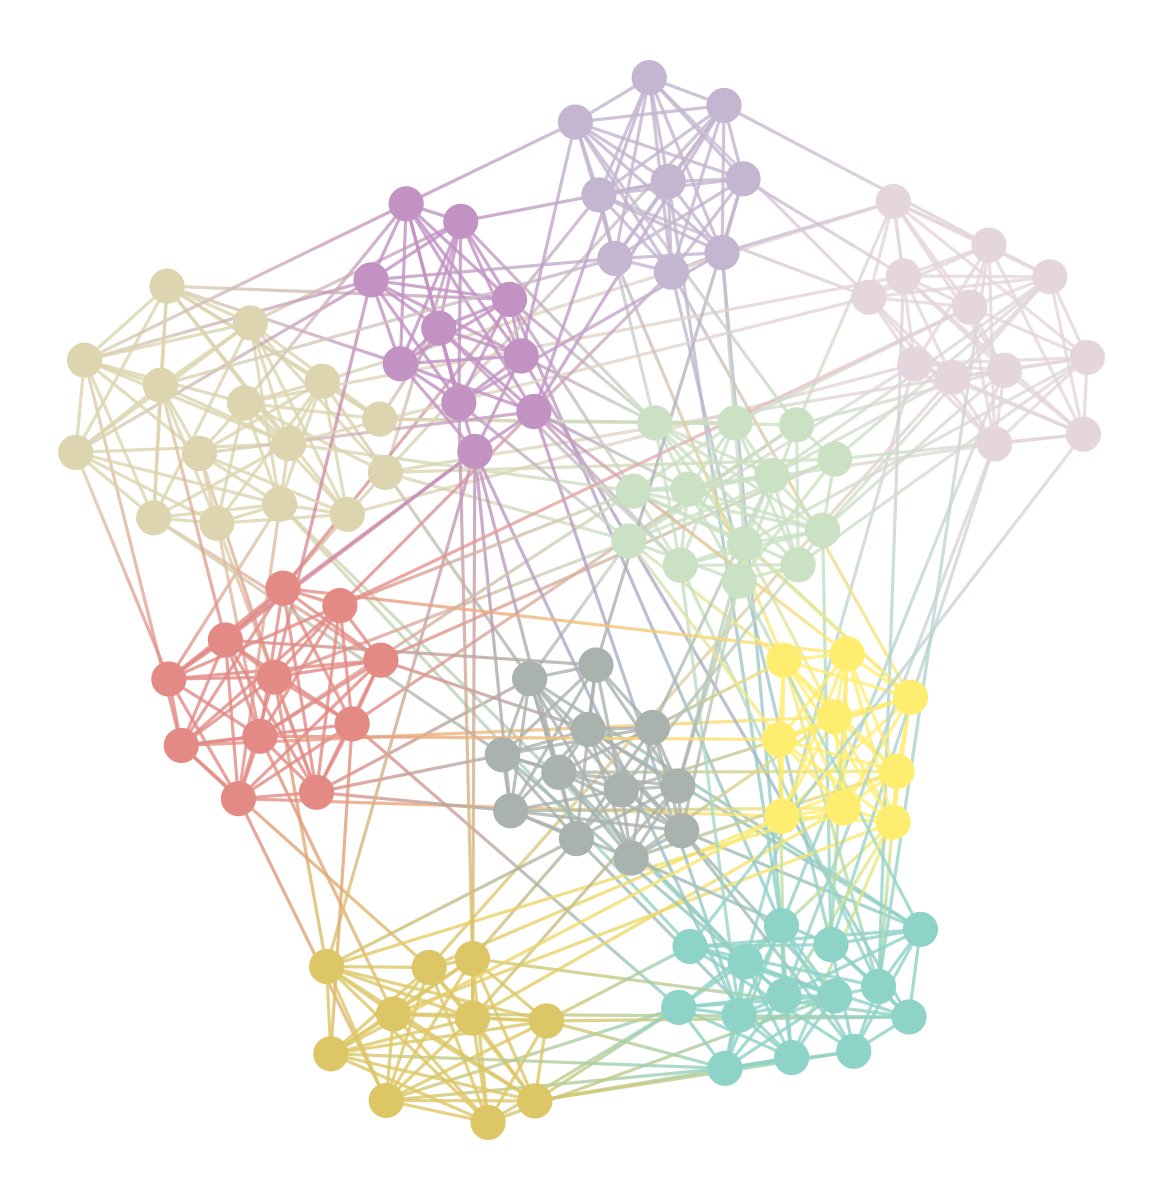
\includegraphics[width=\textwidth]{./figures/assortative.png}
                \footnotesize
                \caption*{Nodes colored by social group}
            \end{figure}
        \end{column}
        \begin{column}{0.6\textwidth}
            $\X_{i \cdot} \in \set{0, 1}^d$ one-hot indicator of social group \\
            \vspace{4mm}
            $B \in [0, 1]^{d \times d}$ between-group friend probabilities \\
            \vspace{4mm}
            Friendships depend on social group and $B$ \\
            \vspace{4mm}
            $\P[\X]{A_{ij} = 1} = \X_{i \cdot} B \X_{j \cdot}^T$ \\
            \vspace{4mm}
            \underline{Social groups $\X$ are latent (i.e., unobserved)} \\
        \end{column}
    \end{columns}
\end{frame}

\begin{frame}{We have very rich and general models for latent social groups}
    \begin{columns}
        \begin{column}{0.4\textwidth}
            \begin{figure}
                \centering
                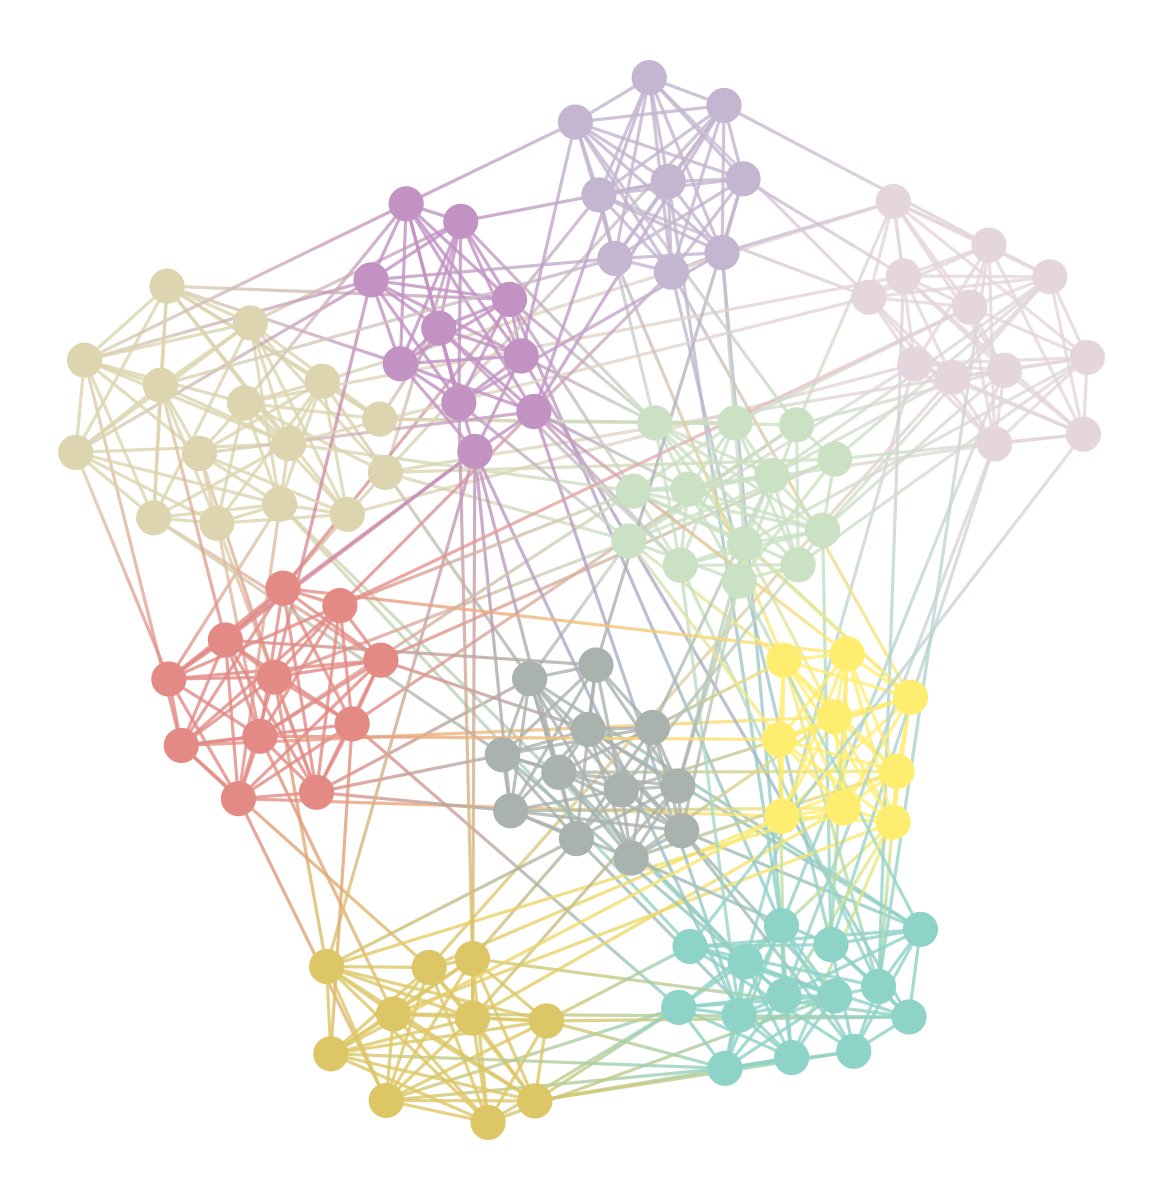
\includegraphics[width=\textwidth]{./figures/assortative.png}
                \footnotesize
                \caption*{Nodes colored by social group}
            \end{figure}
        \end{column}
        \begin{column}{0.6\textwidth}
            \begin{itemize}
                \item Degree-correction
                \item Mixed-membership social groups
                \item Overlapping social groups
                \item Group-specific popularity parameters
            \end{itemize}
            \vspace{4mm}
            \begin{definition}[Random dot product graph]
                $A$ symmetric, weighted adjacency matrix \\
                $A = \X \X^T + E$ \\
                $\X_{1 \cdot}, \dots, \X_{n \cdot} \in \R^{1 \times d}$ i.i.d. latent positions \\
                $E$ independent sub-gamma noise
            \end{definition}
        \end{column}
    \end{columns}
\end{frame}

\begin{frame}{Causal effects on a network decompose into a social and non-social component}
    \begin{figure}
        \centering
        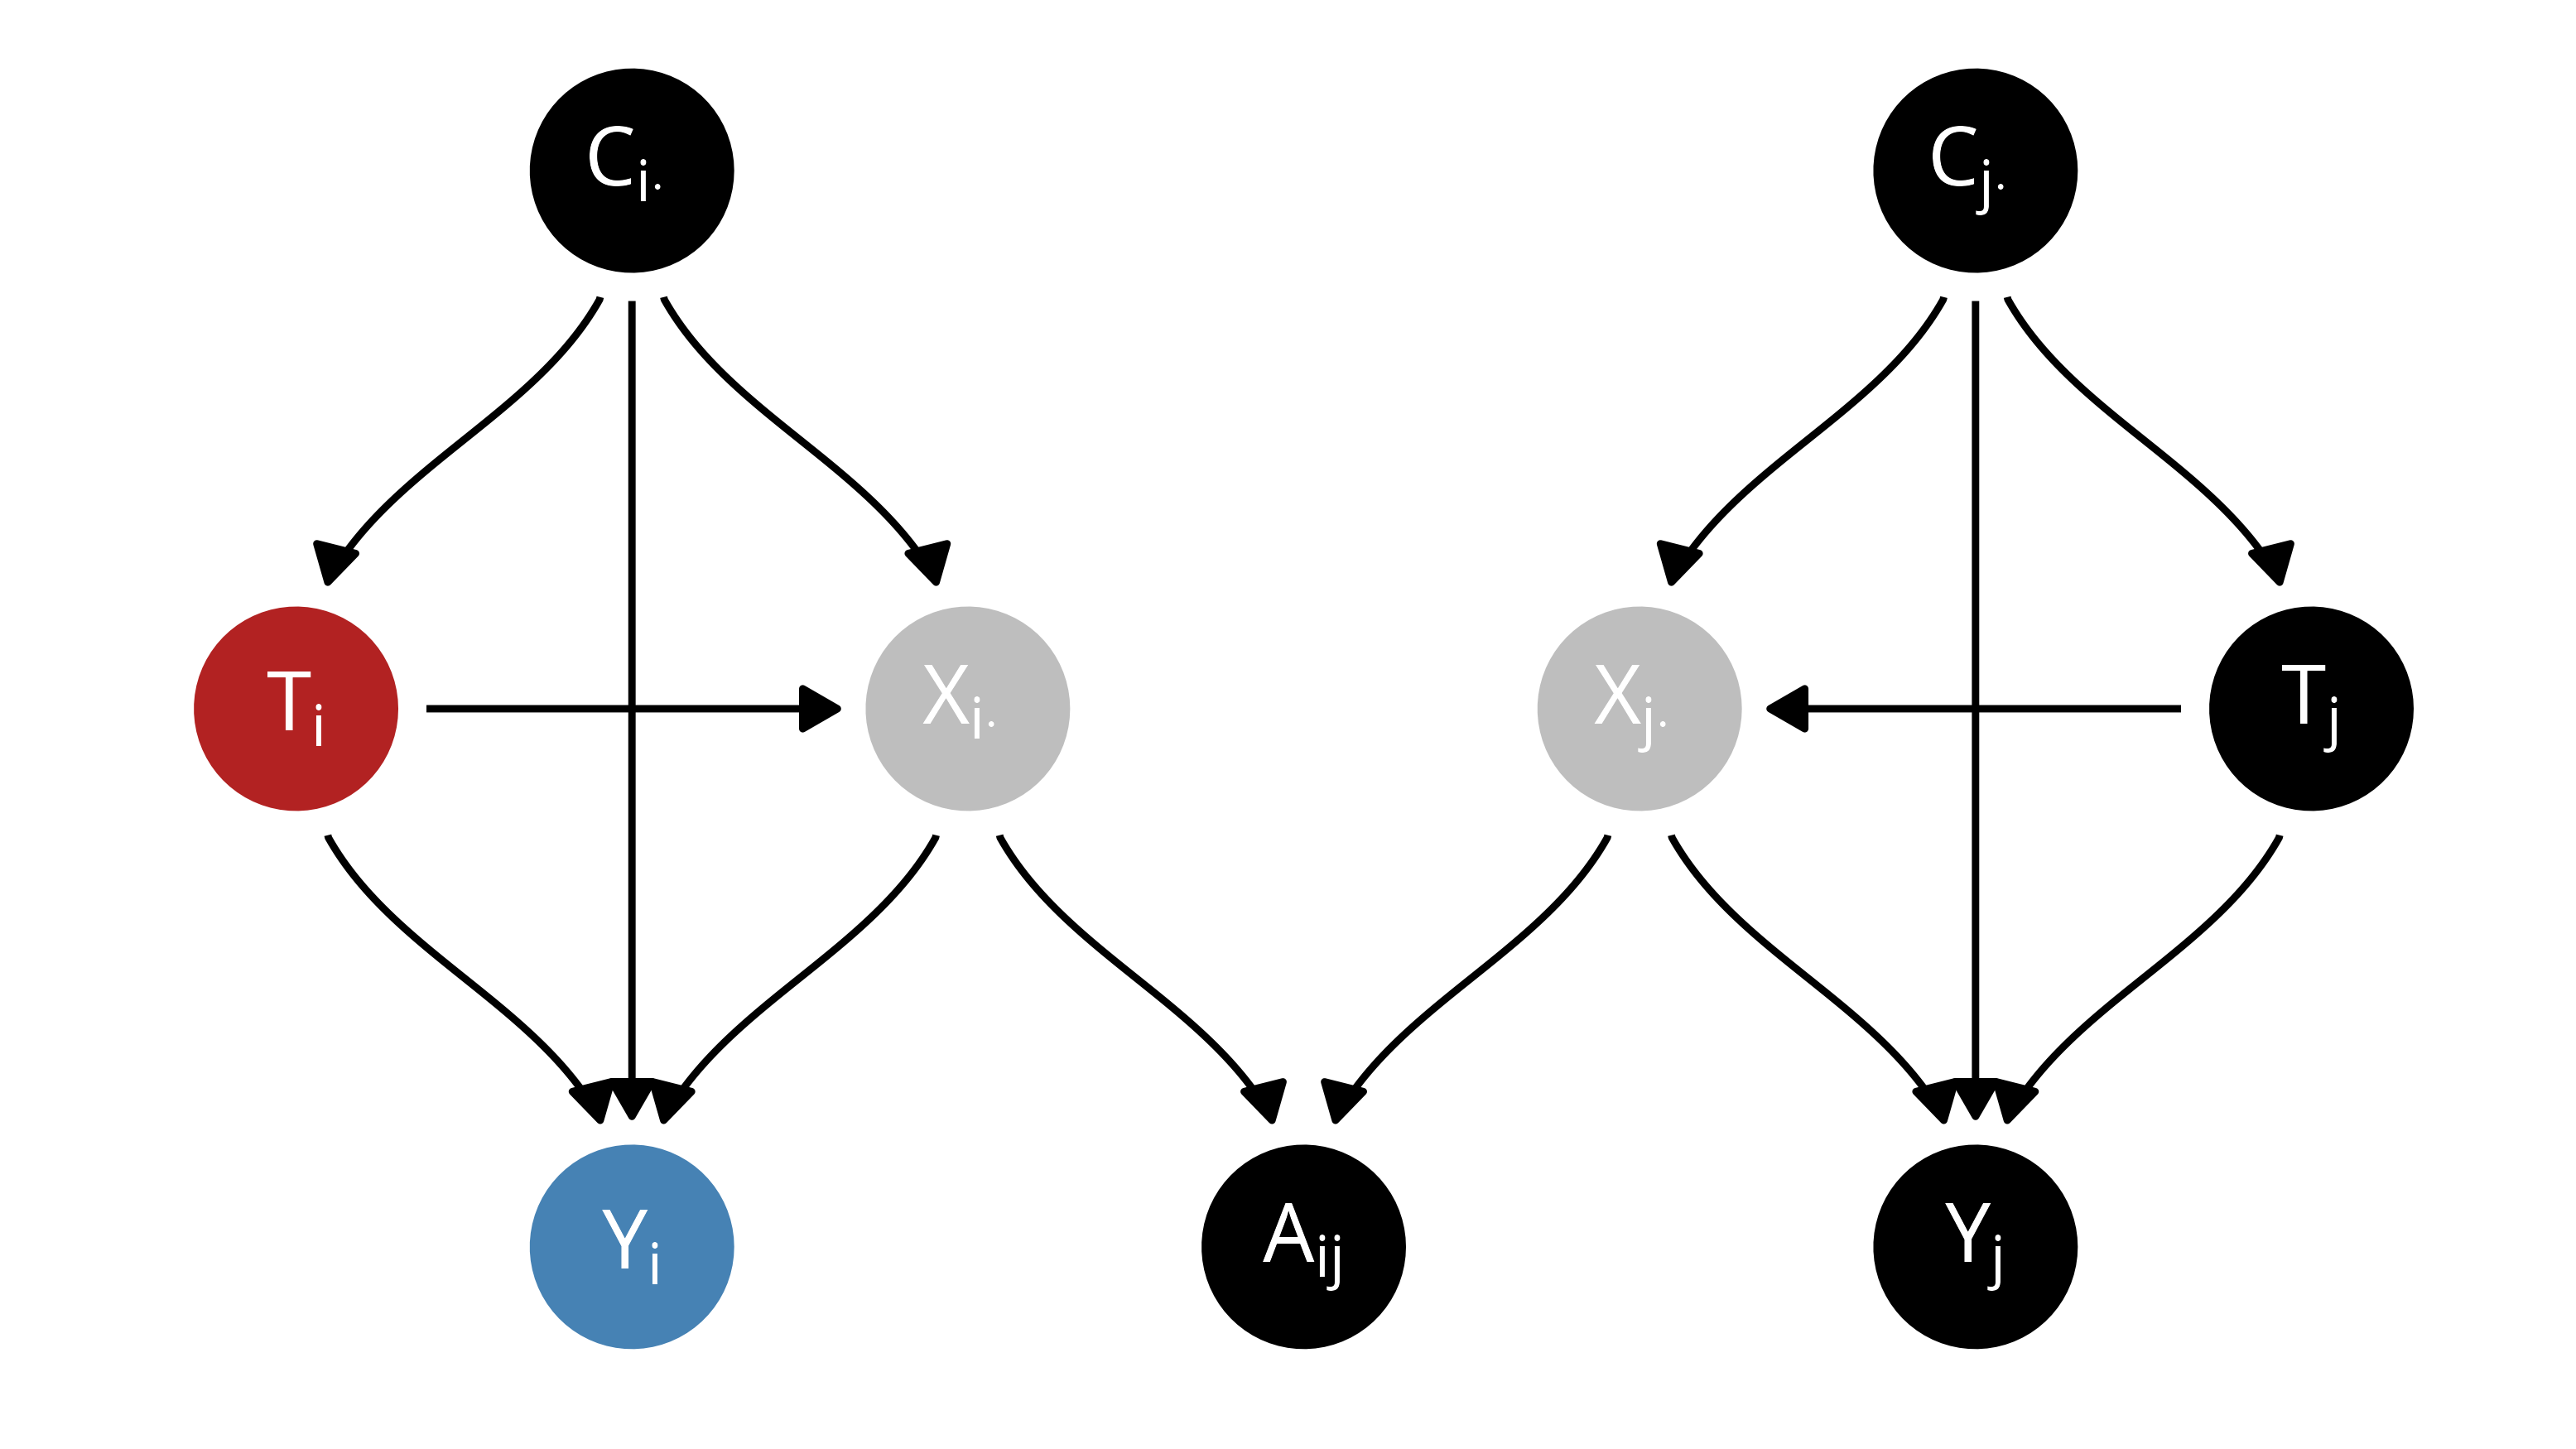
\includegraphics[width=\textwidth]{./figures/dags/homophily-mediating.png}
    \end{figure}
\end{frame}

\begin{frame}{Direct and indirect effects are identified under counterfactual assumptions}
    The random variables $(Y_i, Y_i(t, x), \X_{i \cdot}, \X_{i \cdot}(t), C_{i \cdot}, T_i)$ are independent over $i \in [n]$ and obey the following three properties.
    \begin{enumerate}
        \item Consistency: \vspace{-3mm}
              \begin{equation*} \begin{aligned}
                       & \text{if $T_i = t$, then $\X_{i \cdot}(t) = \X_{i \cdot}$ with probability 1, and}    \\
                       & \text{if $T_i = t$ and $\X_{i \cdot} = x$, then $Y_i(t, x) = Y_i$ with probability 1}
                      \vspace{-2mm}
                  \end{aligned} \end{equation*}
        \item Sequential ignorability:
              \begin{equation*}
                  \set{Y_i(t^*, x), \X_{i \cdot}(t)} \indep T_i \cond C_{i \cdot}
                  ~~~\text{ and }~~~
                  \set{Y_i(t^*, x)} \indep \X_{i \cdot}  \cond T_i = t, C_{i \cdot}
              \end{equation*}
        \item Positivity:
              \begin{equation*}
                  \begin{aligned}
                      \P[T_i, C_{i \cdot}]{x} & > 0 \text{ for each }  x \in \supp(\X_{i \cdot}) \\
                      \P[C_{i \cdot}]{t}      & > 0 \text{ for each }  t \in \supp(T_i)
                  \end{aligned}
              \end{equation*}
    \end{enumerate}
\end{frame}

\begin{frame}{We want to use a regression estimator for direct and indirect effects}
    \begin{block}{Assumption}
        \begin{equation*}
            \begin{aligned}
                \E[T_i, C_{i \cdot}, \X_{i \cdot}]{Y_i}
                 & = \betazero + T_i \betat + C_{i \cdot} \betac + \X_{i \cdot} \betax
                 & \text{outcome model}                                                \\
                \E[T_i, C_{i \cdot}]{\X_{i \cdot}}
                 & = \thetazero + T_i \thetat + C_{i \cdot} \Thetac
                 & \text{mediator model}
            \end{aligned}
        \end{equation*}
    \end{block}
    \begin{block}{Fact: semi-parametric identification of natural mediated effects}
        Under previous assumption, when natural direct and indirect effect are non-parametrically identified, we have
        \begin{equation*}
            \begin{aligned}
                \nde & = \betat            \\
                \nie & = \thetat \, \betax
            \end{aligned}
        \end{equation*}
    \end{block}
    \centering
    \textbf{Problem}: We don't see the latent social groups $\X$, can't fit regressions
\end{frame}

\begin{frame}{Latent positions $X$ can be estimated via principal components analysis}
    \begin{definition}[ASE]
        Given a network $A$, the $d$-dimensional \emph{adjacency spectral embedding} of $A$ is
        \begin{align*}
            \Xhat = \Uhat \Shat^{1/2}
        \end{align*}
        \noindent where $\Uhat \Shat \Uhat^T$ is the rank-$d$ truncated singular value decomposition of $A$.
    \end{definition}
    \begin{lemma}
        Under a suitable network model, there is a $d \times d$ orthogonal matrix $Q$ such that
        \begin{equation*}
            \max_{i \in [n]} \, \norm*{\Xhat_{i \cdot} - \X_{i \cdot} Q} = \op{1}.
        \end{equation*}
    \end{lemma}
\end{frame}

\begin{frame}{Estimated latent positions can plug directly into ordinary least squares}
    Let $\Dhat = \begin{bmatrix} 1 & T & C  & \Xhat \end{bmatrix} \in \R^{n \times (2 + p + d)}$ and $\Wfull = \begin{bmatrix} 1 & T & C \end{bmatrix} \in \R^{n \times (p + 2)}$.
    \begin{equation*}
        \begin{bmatrix}
            \betazerohat \\
            \betathat    \\
            \betachat    \\
            \betaxhat
        \end{bmatrix}
        = \paren*{\Dhat^T \Dhat}^{-1} \Dhat^T Y
        \quad \text{and} \quad
        \Thetahat
        = \paren*{\Wfull^T \Wfull}^{-1} \Wfull^T \Xhat.
    \end{equation*}
    \begin{align*}
        \ndehat = \betathat \quad \text{and} \quad \niehat = \thetathat \, \betaxhat
    \end{align*}
\end{frame}

\begin{frame}{Ordinary least squares regression estimates are asymptotically normal}
    \begin{theorem}
        Under a suitably well-behaved network model and some moments conditions on regression errors, there is an unknown orthogonal matrix $Q$ such that
        \begin{equation*}
            \begin{aligned}
                \sqrt{ n } \,
                 & \Sigmahatbeta^{-1/2}
                \begin{pmatrix}
                    \betawhat - \betaw \\
                    Q \, \betaxhat - \betax
                \end{pmatrix}
                \to
                \Normal{0}{I_d}, and     \\
                \sqrt{ n } \,
                 & \Sigmahattheta^{-1/2}
                \begin{pmatrix}
                    \vecc \paren*{\Thetahat \, Q^T} - \Thetavec
                \end{pmatrix}
                \to
                \Normal{0}{I_{p d}}.
            \end{aligned}
        \end{equation*}
        \noindent where $\Sigmahattheta^{-1/2}$ and $\Sigmahatbeta^{-1/2}$ are the typical heteroscedastic robust covariance estimators, with $\Xhat$ plugged in for $\X$.
    \end{theorem}

    \centering
    Note: theory requires consistent estimate of latent dimension $d$
\end{frame}

\begin{frame}{Aside: our regression results are substantially more general than similar work}
    \begin{itemize}
        \item Network can be weighted, rather than binary
        \item No parametric assumptions on edge noise
        \item No parametric assumptions on regression errors
        \item Regression errors can be heteroscedastic
        \item Can model latent positions as outcomes
    \end{itemize}
    Principle components + ordinary least squares is a very general, distributionally agnostic tool for network regression \\
    \vspace{2mm}
    \underline{Folklore}: similar results hold for asymmetric $A$, rectangular $A$, bipartite $A$, graph Laplacian embeddings rather than adjacency matrix embeddings, general regression $M$-estimators other than ordinary least squares
\end{frame}

\begin{frame}{Causal estimators are asymptotically normal}
    \vspace{2mm}
    \begin{theorem}
        Under the same statistical assumptions as before, plus counterfactual assumptions required for causal identification,
        \begin{align*}
            \sqrt{n \, \sigmahatnde} \paren*{\ndehat - \nde}
             & \to
            \Normal{0}{1}, \text { and } \\
            \sqrt{n \, \sigmahatnie} \paren*{\niehat - \nie}
             & \to
            \Normal{0}{1}.
        \end{align*}
        \noindent where $\sigmahatnde$ and $\sigmahatnie$ are rather unfriendly variance estimators derived via the delta method and the previous theorem.
    \end{theorem}

    \begin{block}{A useful cancellation}
        \begin{equation*}
            \niehat = \thetathat \, \betaxhat \to \thetat \, Q^T Q \, \betax = \thetat \betax = \nie
        \end{equation*}
    \end{block}
\end{frame}

\begin{frame}{Simulations show that overestimating the embedding dimension is okay}
    \centering
    \begin{figure}
        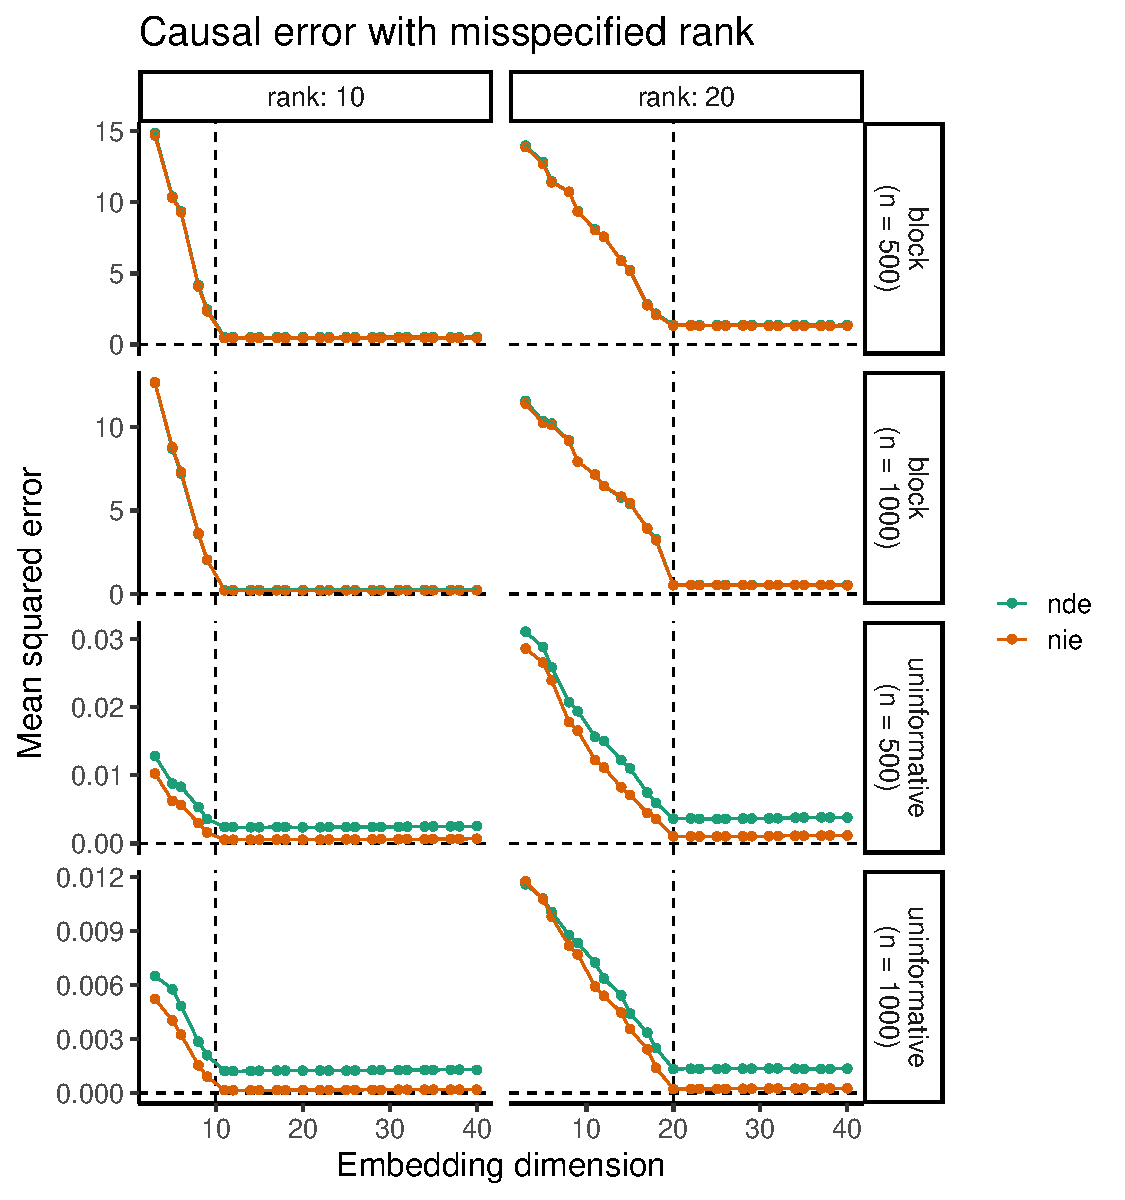
\includegraphics[width=0.5\textwidth]{figures/misspecification/loss_average.pdf}
    \end{figure}
\end{frame}

\begin{frame}{Motivation: understand causes of teenage smoking \citep{michell1996}}
    \begin{columns}
        \centering
        \begin{column}{0.55\textwidth}
            \begin{figure}
                \centering
                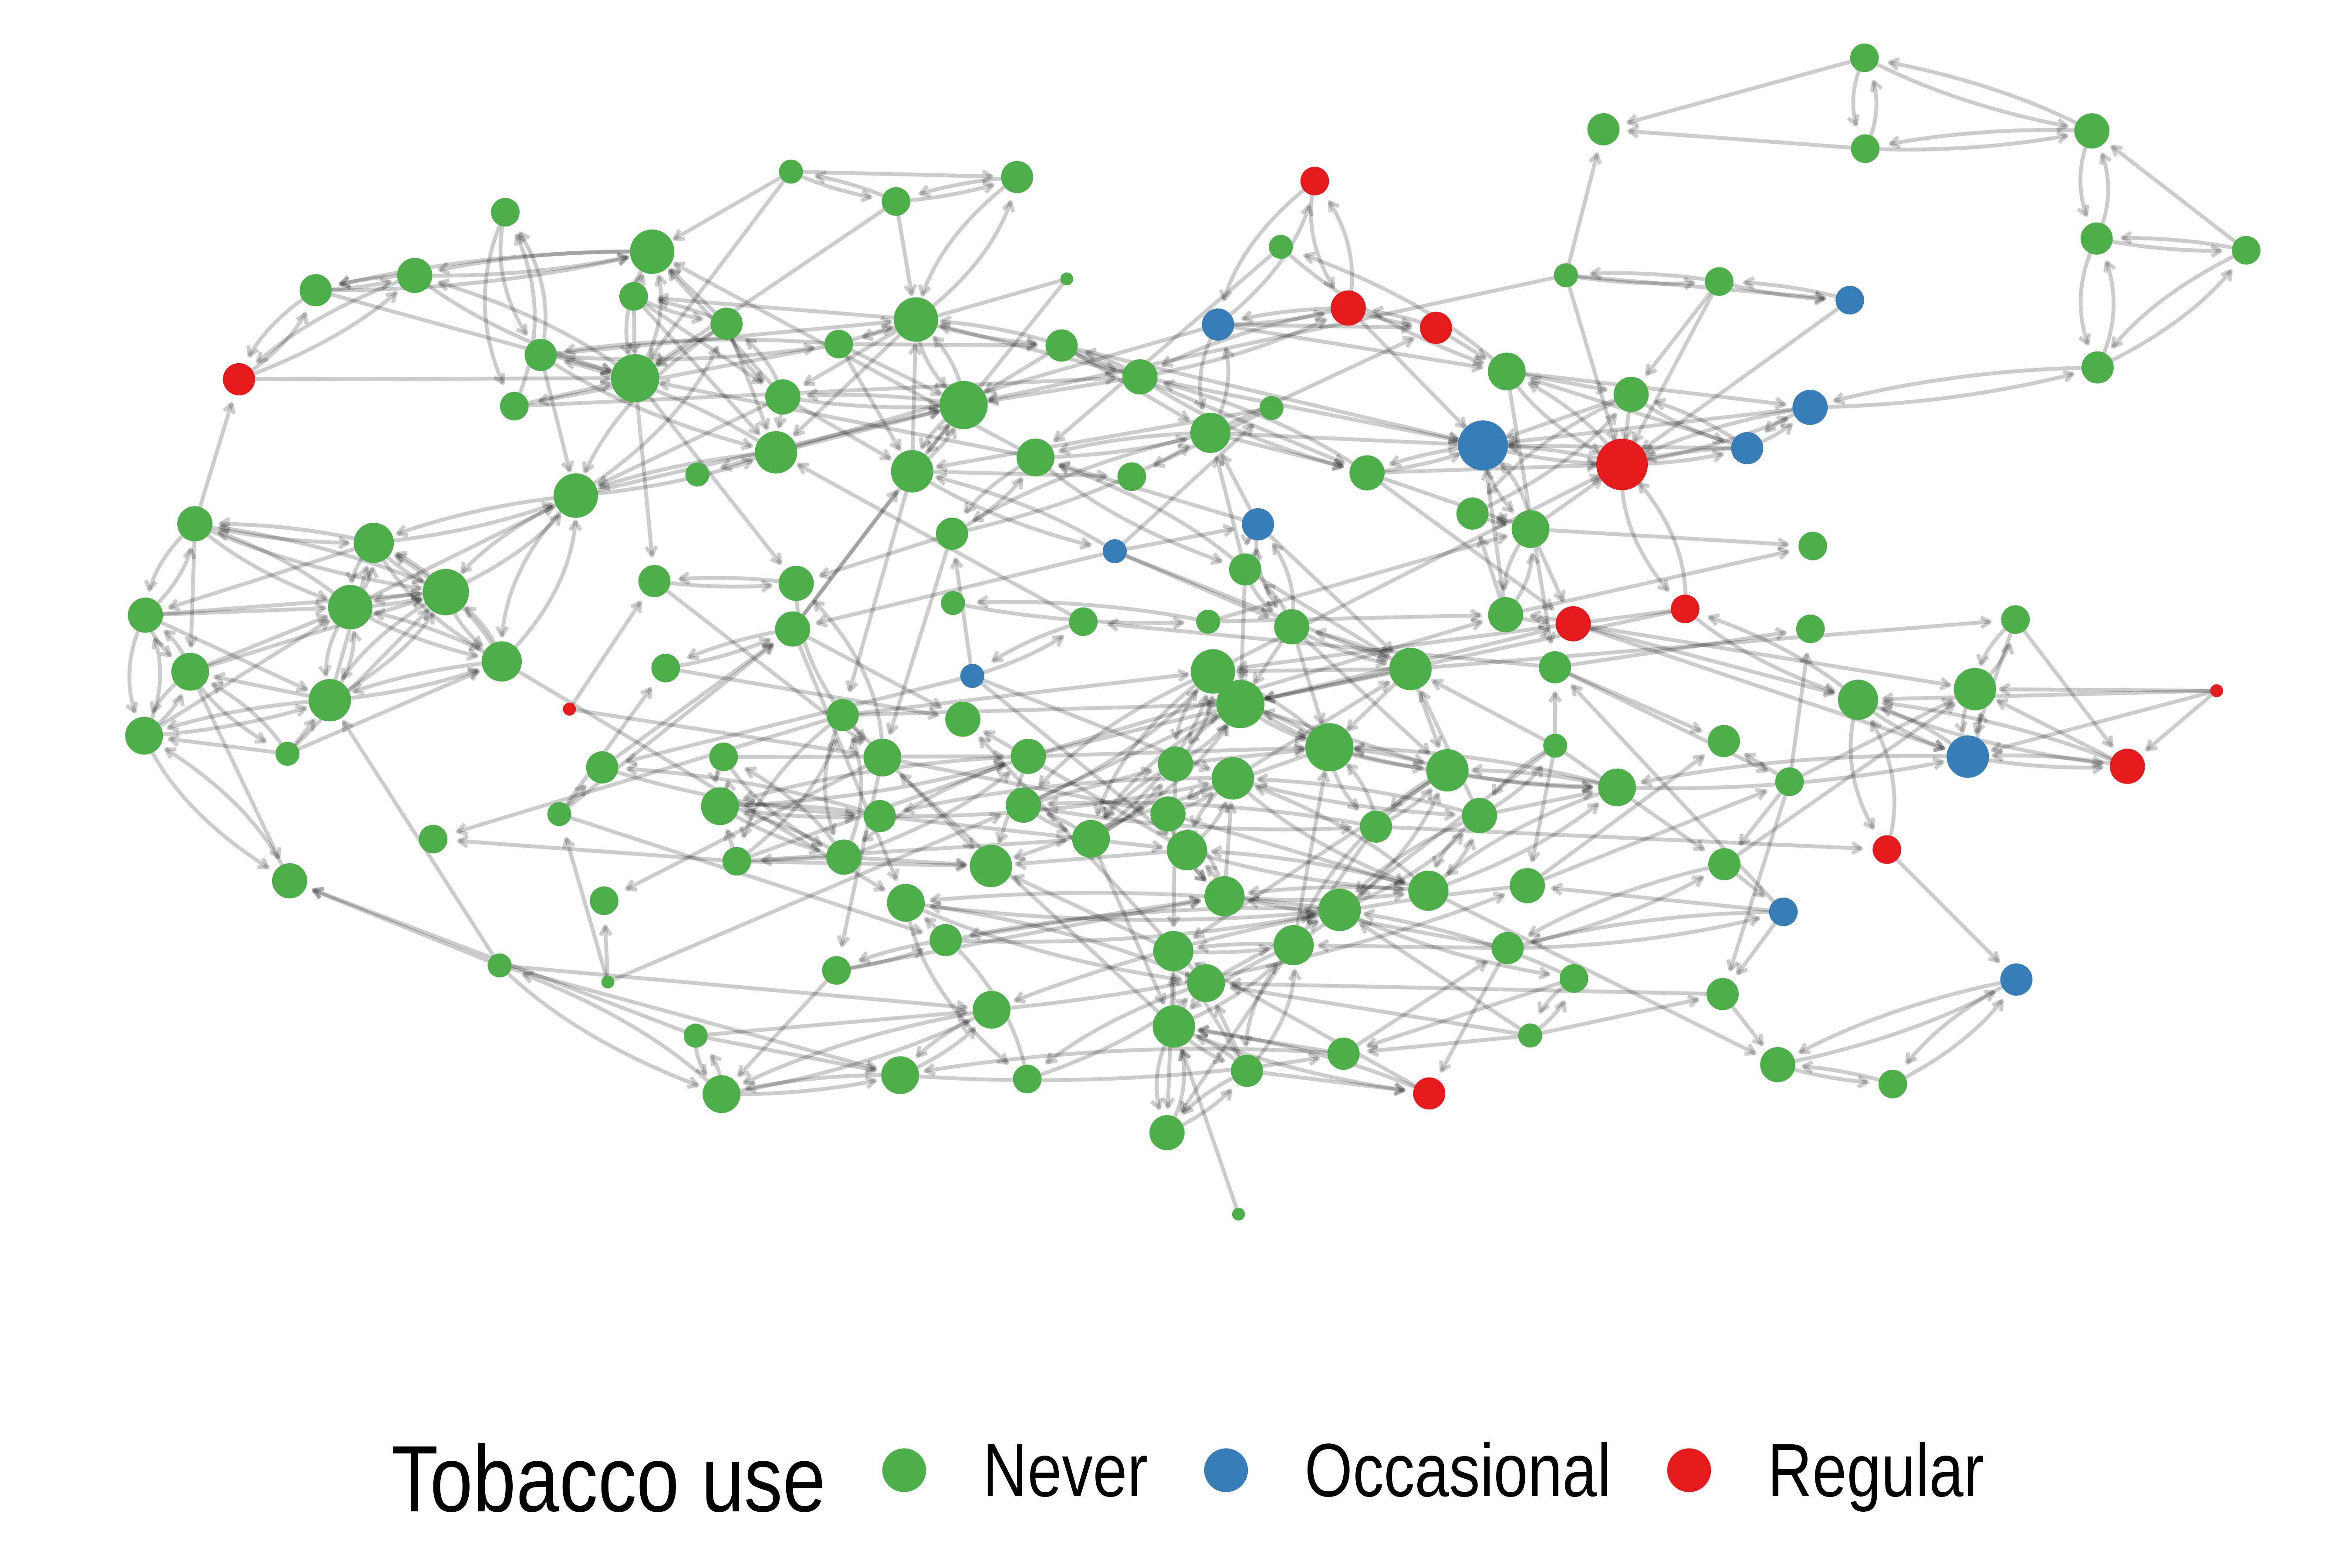
\includegraphics[width=1.05\textwidth]{figures/glasgow/tobacco.png}
            \end{figure}
        \end{column}
        \begin{column}{0.5\textwidth}
            \begin{itemize}
                \item 129 middle-schoolers in Glasgow
                \item {\bf Social network} based on self-reported friendships
                \item {\bf Auxiliary data:} spending money, leisure activities
                \item {\bf Demographics:} sex, age
                \item {\bf Behavior:} alcohol, cannabis and tobacco use
            \end{itemize}
        \end{column}
    \end{columns}
    \vspace{2mm}
    \centering
    \textbf{Question:} how does sex influence tobacco use?
\end{frame}

\begin{frame}{Application to Glasgow data}
    \begin{columns}
        \centering
        \begin{column}{0.55\textwidth}
            We fit the following regressions
            \vspace{2mm}
            \begin{equation*}
                \begin{aligned}
                    \texttt{smoking} & \sim \texttt{sex + age + church + Xhat} \\
                    \texttt{Xhat}    & \sim \texttt{sex + age + church}.
                \end{aligned}
            \end{equation*}
        \end{column}
        \begin{column}{0.5\textwidth}
            \begin{itemize}
                \item 129 middle-schoolers in Glasgow
                \item {\bf Social network} based on self-reported friendships
                \item {\bf Auxiliary data:} spending money, leisure activities
                \item {\bf Demographics:} sex, age
                \item {\bf Behavior:} alcohol, cannabis and tobacco use
            \end{itemize}
        \end{column}
    \end{columns}
    \vspace{2mm}
    \centering
    \textbf{Question:} how does sex influence tobacco use?
\end{frame}

\begin{frame}{Application to Glasgow data}
    \begin{columns}
        \begin{column}{0.75\textwidth}
            \begin{figure}
                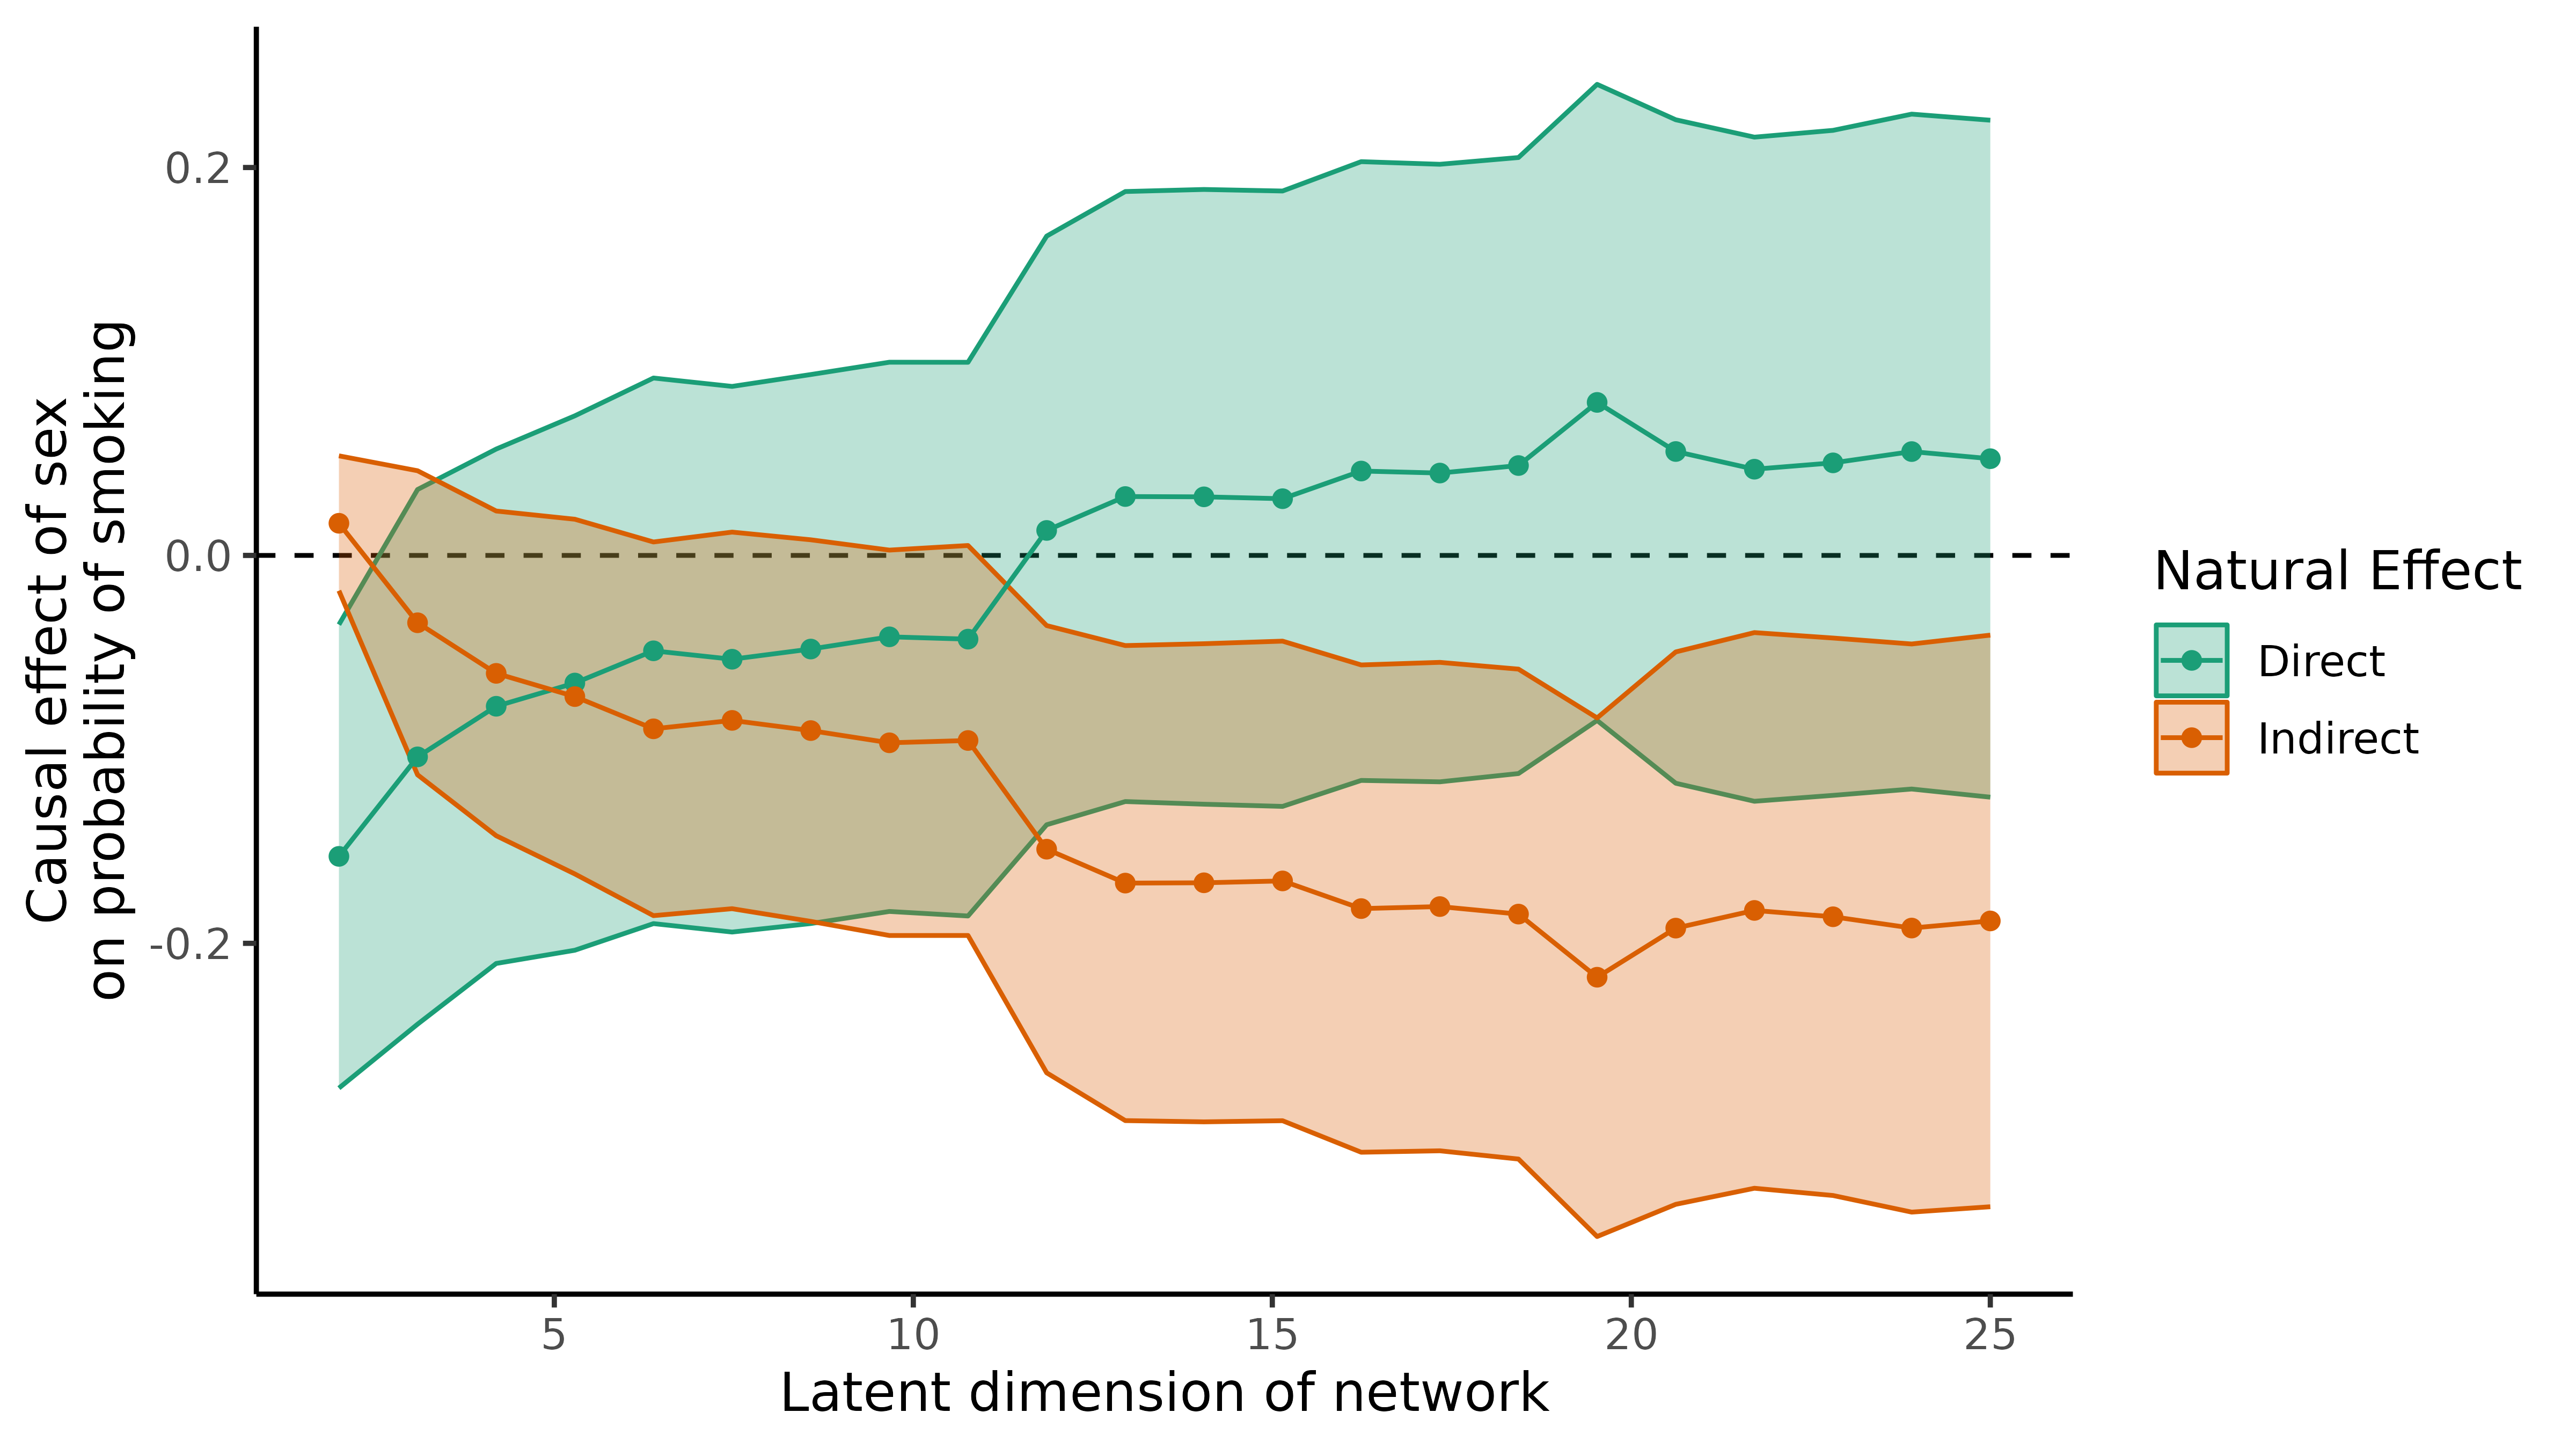
\includegraphics[width=1.05\textwidth]{figures/glasgow/effects.png}
            \end{figure}
        \end{column}
        \begin{column}{0.28\textwidth}
            \footnotesize
            \begin{itemize}
                \item No direct effect of sex on smoking
                \item Indirect social effect leads girls to smoke more
                \item Interventions should try to disrupt social mechanisms
            \end{itemize}
        \end{column}
    \end{columns}
\end{frame}

\begin{frame}{Takeaway 1: network regression is straightforward and easy}
    Use ordinary least squares and principal components analysis to fit models \\
    \begin{equation*}
        \begin{aligned}
            \E[T_i, C_{i \cdot}, \X_{i \cdot}]{Y_i}
             & = \betazero + T_i \betat + C_{i \cdot} \betac + \X_{i \cdot} \betax \\
            \E[T_i, C_{i \cdot}]{\X_{i \cdot}}
             & = \thetazero + T_i \thetat  + C_{i \cdot} \Thetac                   \\
        \end{aligned}
    \end{equation*}
    No distributional assumptions needed!
\end{frame}

\begin{frame}{Takeaway 2: network embeddings might not be confounders}
    \centering
    \textbf{Current practice}: estimate $\Xhat$, blindly throw into regression to control for ``confounding'' \\
    \vspace{4mm}
    This will lead to overcontrol bias!
\end{frame}

\begin{frame}{Takeaway 2: network embeddings might not be confounders}
    When latent positions are confounders:
    \begin{equation*}
        \begin{aligned}                                                    \\
            \E[T_i, C_{i \cdot}, \X_{i \cdot}]{Y_i}
             & = \betazero + T_i \underbrace{\betat}_{\substack{\text{average} \\ \text{treatment} \\ \text{effect}}} + C_{i \cdot} \betac + \X_{i \cdot} \betax
        \end{aligned}
    \end{equation*}

    When latent positions are mediators:
    \begin{equation*}
        \begin{aligned}                                                    \\
            \E[T_i, C_{i \cdot}, \X_{i \cdot}]{Y_i}
             & = \betazero + T_i \underbrace{\betat}_{\substack{\text{natural}     \\ \text{direct} \\ \text{effect}}} + C_{i \cdot} \betac + \X_{i \cdot} \underbrace{\betax}_{\substack{\text{effect of} \\ \text{$X$ on $Y$}}}  \\
            \E[T_i, C_{i \cdot}]{\X_{i \cdot}}
             & = \thetazero + T_i \underbrace{\thetat}_{\substack{\text{effect of} \\ \text{$T$ on $X$}}}  + C_{i \cdot} \Thetac
        \end{aligned}
    \end{equation*}
\end{frame}

\begin{frame}{Thank you! Questions?}
    Future work:
    \begin{itemize}
        \item Varimax rotation for improved interpretability
        \item Peer effects
    \end{itemize}
    \vspace{4mm}
    \begin{block}{Pre-print}
        Alex Hayes, Mark M. Fredrickson, and Keith Levin. “Estimating Network-Mediated Causal Effects via Spectral Embeddings.” arXiv, April 14, 2023. \url{https://arxiv.org/abs/2212.12041}.
    \end{block}
    \centering
    Contact info \& slides: \href{www.alexpghayes.com}{https://www.alexpghayes.com}
\end{frame}

\section{Appendix}
\appendix


\begin{frame}{Can we include peer effects in the outcome regression model?}
    \begin{equation*}
        \begin{aligned}
            Y_i
            = \betazero + T_i \betat + C_{i \cdot} \betac + \X_{i \cdot} \betax +
            \underbrace{\beta_\text{gt} \sum_{j \neq i} \frac{A_{ij} T_j}{\sum_i A_{ij}}}_\text{interference} +
            \underbrace{\beta_\text{gy} \sum_{j \neq i} \frac{A_{ij} Y_j}{\sum_i A_{ij}}}_\text{``contagion''} +
            \varepsilon_i
        \end{aligned}
    \end{equation*}
    \begin{itemize}
        \item Identifying peer effects in these models is very nuanced
              \begin{itemize}
                  \item Not one but two forthcoming manuscripts about this
              \end{itemize}
        \item When peer effects are identified, ordinary least squares sometimes works
        \item When peer effects are unidentified, typically due to aliasing with $\betax$ or $\betazero$
              \begin{itemize}
                  \item Aliasing might occur only in the asymptotic limit
                  \item Might already be accounting for peer effects via aliasing
              \end{itemize}
    \end{itemize}
\end{frame}

\begin{frame}{Intervention has downstream impacts on network structure}
    \begin{columns}
        \begin{column}{0.5\textwidth}
            \begin{figure}
                \centering
                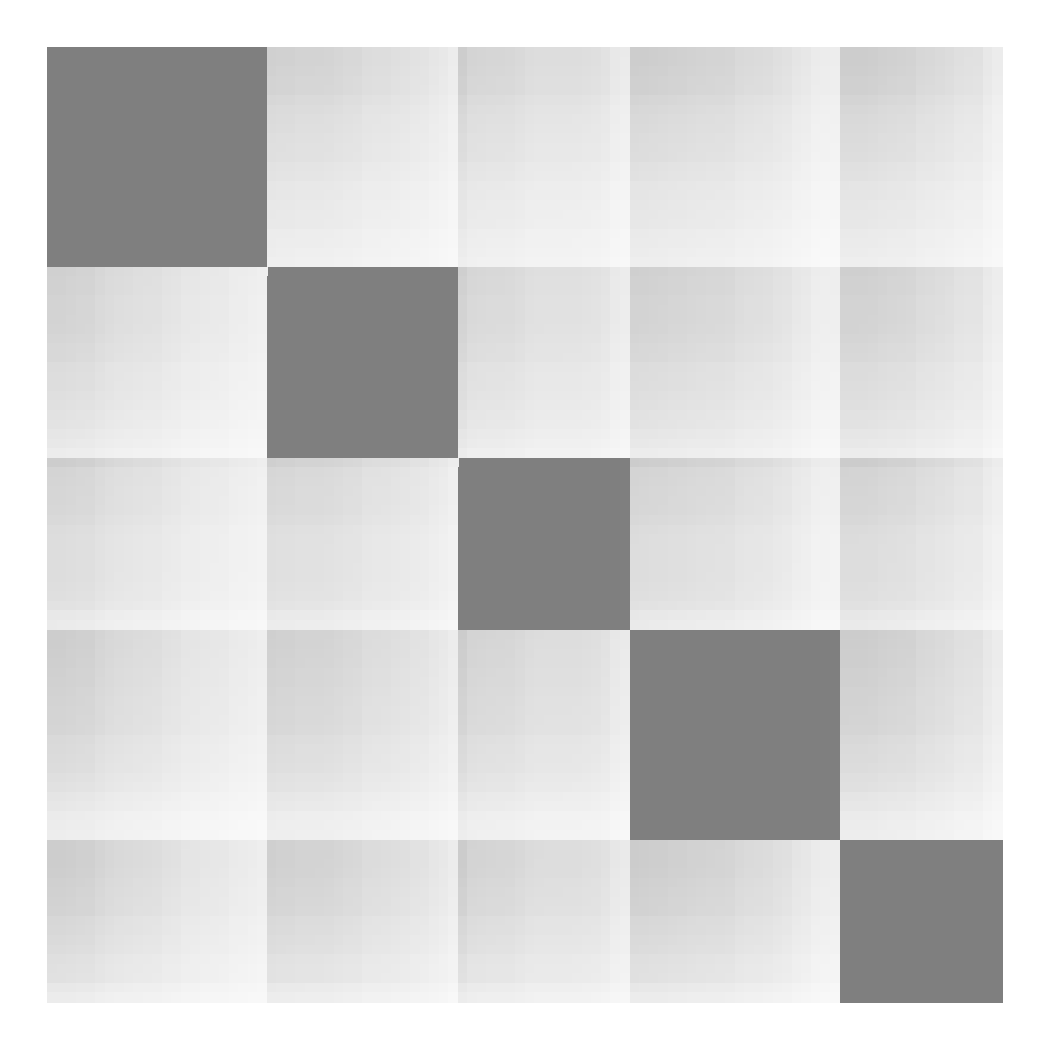
\includegraphics[width=0.8\textwidth]{figures/canonical-intervention/expected-a-pre-trt.pdf}
                \caption{$\E[X]{A}$ prior to intervention.}
            \end{figure}
        \end{column}
        \begin{column}{0.5\textwidth}
            \begin{figure}
                \centering
                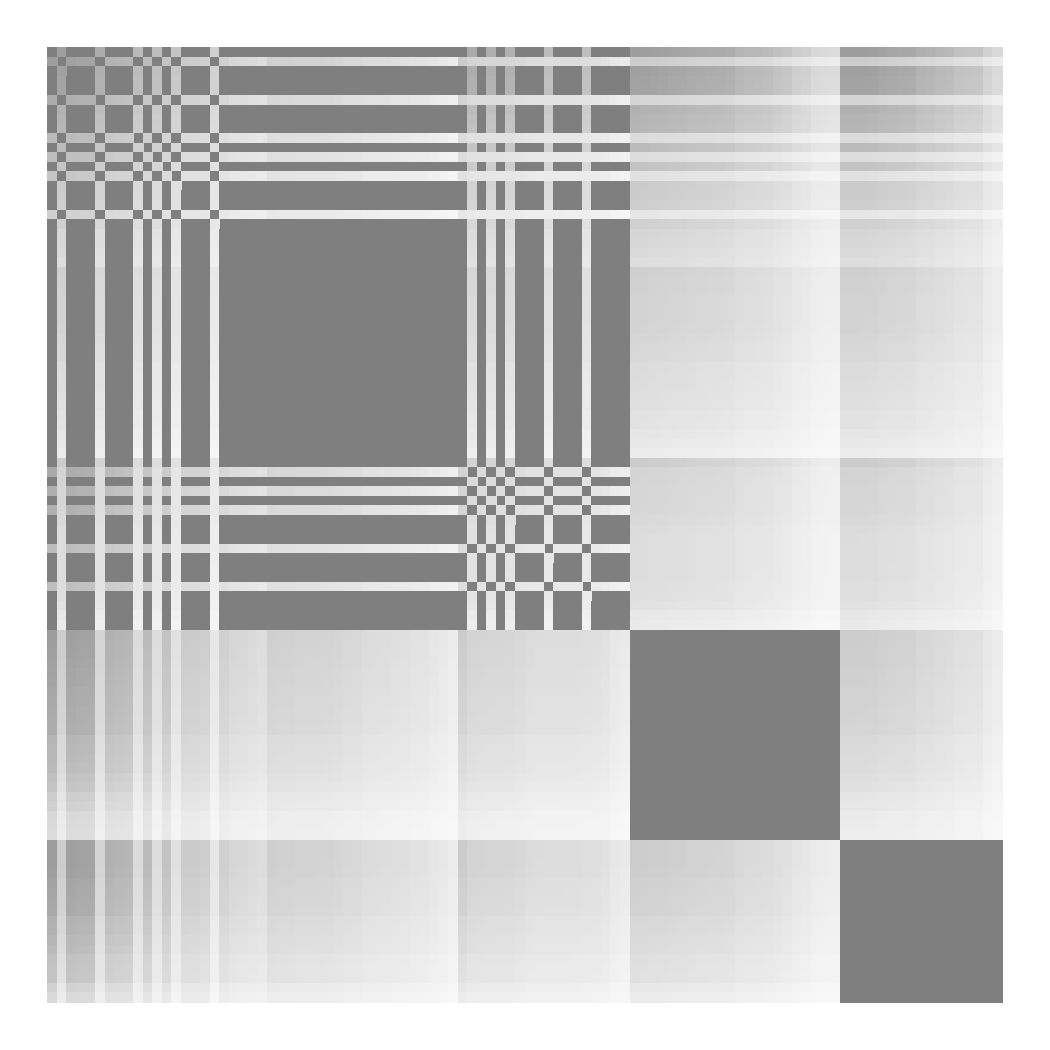
\includegraphics[width=0.8\textwidth]{figures/canonical-intervention/expected-a-post-trt.pdf}
                \caption{$\E[X]{A}$ after intervention.}
            \end{figure}
        \end{column}
    \end{columns}
\end{frame}

\begin{frame}{Intervention has downstream impacts on network structure}
    \begin{columns}
        \begin{column}{0.5\textwidth}
            \begin{figure}
                \centering
                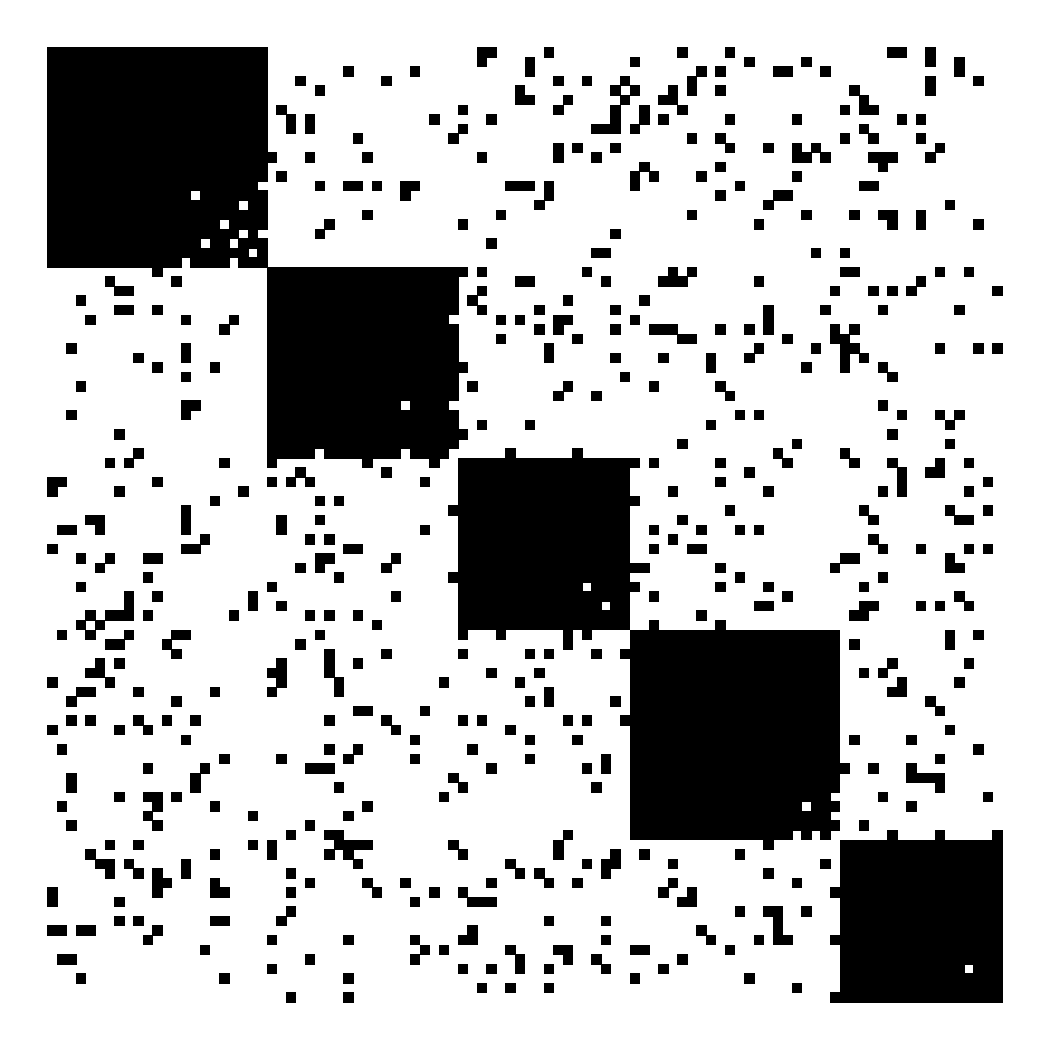
\includegraphics[width=0.8\textwidth]{figures/canonical-intervention/a-untreated.pdf}
                \caption{Realized network before intervention}
            \end{figure}
        \end{column}
        \begin{column}{0.5\textwidth}
            \begin{figure}
                \centering
                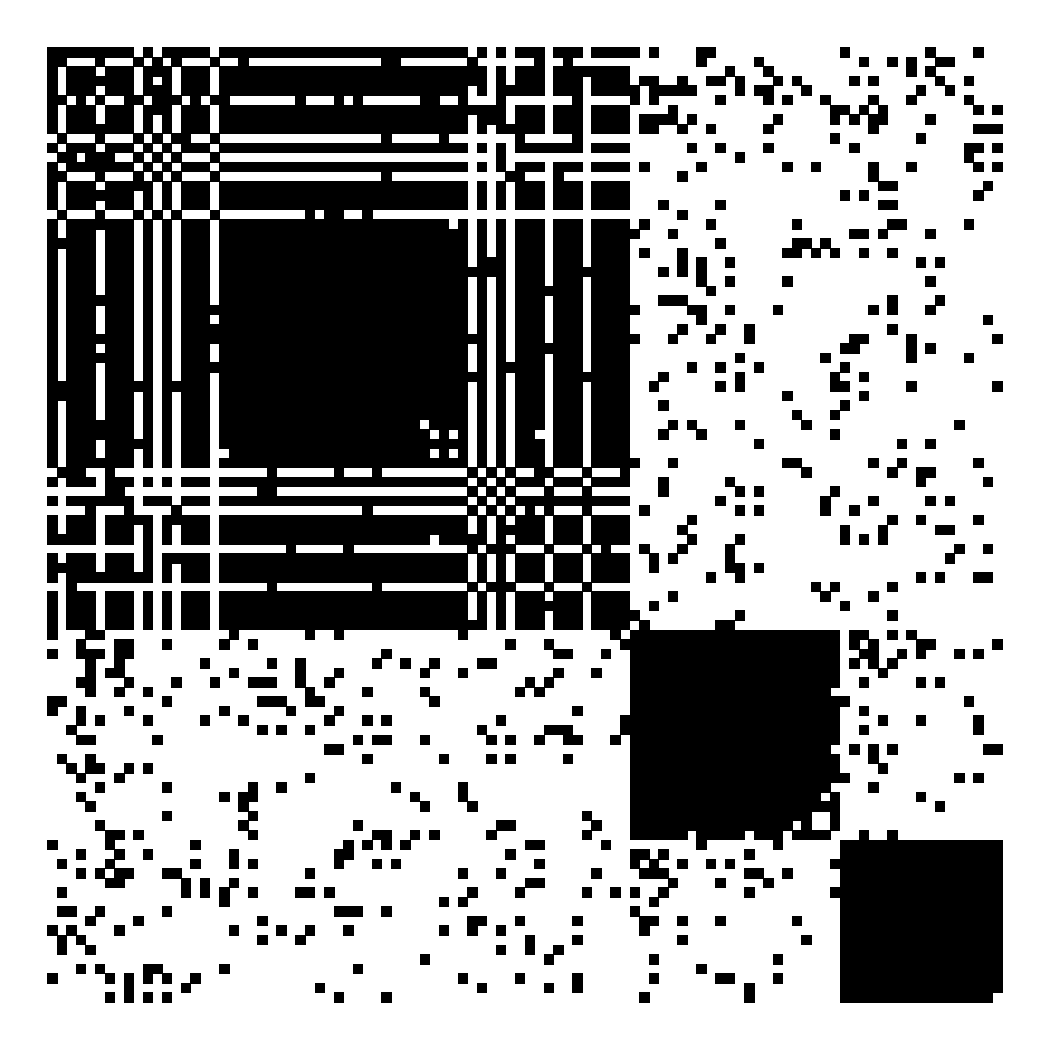
\includegraphics[width=0.8\textwidth]{figures/canonical-intervention/a-treated.pdf}
                \caption{Realized network after intervention}
            \end{figure}
        \end{column}
    \end{columns}
\end{frame}

\begin{frame}{Interpreting interventions on social group membership}
    Treatment $T_i$ is allowed to cause:
    \begin{itemize}
        \item Changes in popularity within a group
        \item Movement to a new friend group
        \item Becoming a member of a new friend group while remaining in current friend group
        \item Friendships becoming more or less likely between distinct friend groups
        \item Combinations of the above
    \end{itemize}
\end{frame}

\bibliographystyle{chicago}
\bibliography{2024-06-17-netsci}

\end{document}